\documentclass{book}
\usepackage{fontspec}
\setmainfont{STIX Two Text}

%PACKAGES
\iffalse
Here are the packages that I use
\fi

\usepackage{blindtext, hyperref, verbatim, minted, graphicx, amssymb, textcomp, enumerate, tcolorbox, newunicodechar, textgreek, wasysym, tipa, eso-pic, lipsum, bbold, dsfont}
\usepackage[margin=1.3in]{geometry}
\usepackage{longtable}
\usepackage{newunicodechar}
\usepackage{amsthm}
\usepackage{tikz}
\usepackage{tikz-cd}




%ENVIRONMENTS

%Here I define some common environments. I use definitions, theorems, examples, and lemmas.


\theoremstyle{definition}
\newtheorem{definition}{Definition}
\newtheorem{theorem}{Theorem}
\newtheorem{example}{Example}
\newtheorem{lemma}{Lemma}


\newunicodechar{ₙ}{${}_{n}$}

\newunicodechar{𝓓}{$\mathcal{D}$}
\newunicodechar{∂}{$\partial$}
\newunicodechar{∇}{\raisebox{-0.05cm}{$\nabla$}}

%\newunicodechar{π⃗}{$\stackrel{\arr}{\pi}$}

\newunicodechar{×}{$\times$}
\newunicodechar{→}{$\rightarrow$}
\newunicodechar{⟨}{$\langle$}
\newunicodechar{⟩}{$\rangle$}
\newunicodechar{↦}{$\mapsto$}
\newunicodechar{∧}{$\wedge$}
\newunicodechar{∨}{$\vee$}
\newunicodechar{∃}{$\exists$}
\newunicodechar{∀}{$\forall$}
\newunicodechar{¬}{$\neg$}
\newunicodechar{ᵃ}{${}^{\texttt{a}}$}
\newunicodechar{ᵇ}{${}^{\texttt{b}}$}
\newunicodechar{ᶜ}{${}^{\texttt{c}}$}
\newunicodechar{ᵈ}{${}^{\texttt{d}}$}
\newunicodechar{ᵉ}{${}^{\texttt{e}}$}
\newunicodechar{ᶠ}{${}^{\texttt{f}}$}
\newunicodechar{ᵍ}{${}^{\texttt{g}}$}
\newunicodechar{ʰ}{${}^{\texttt{h}}$}
\newunicodechar{ⁱ}{${}^{\texttt{i}}$}
\newunicodechar{ʲ}{${}^{\texttt{j}}$}
\newunicodechar{ᵏ}{${}^{\texttt{k}}$}
\newunicodechar{ˡ}{${}^{\texttt{l}}$}
\newunicodechar{ᵐ}{${}^{\texttt{m}}$}
\newunicodechar{ⁿ}{${}^{\texttt{n}}$}
\newunicodechar{ᵒ}{${}^{\texttt{o}}$}
\newunicodechar{ᵖ}{${}^{\texttt{p}}$}
\newunicodechar{ʳ}{${}^{\texttt{r}}$}
\newunicodechar{ˢ}{${}^{\texttt{s}}$}
\newunicodechar{ᵗ}{${}^{\texttt{t}}$}
\newunicodechar{ᵘ}{${}^{\texttt{u}}$}
\newunicodechar{ᵛ}{${}^{\texttt{v}}$}
\newunicodechar{ʷ}{${}^{\texttt{w}}$}
\newunicodechar{ˣ}{${}^{\texttt{x}}$}
\newunicodechar{ʸ}{${}^{\texttt{y}}$}
\newunicodechar{ᶻ}{${}^{\texttt{z}}$}
\newunicodechar{⁰}{${}^{\texttt{0}}$}
\newunicodechar{¹}{${}^{\texttt{1}}$}
\newunicodechar{²}{${}^{\texttt{2}}$}
\newunicodechar{³}{${}^{\texttt{3}}$}
\newunicodechar{⁴}{${}^{\texttt{4}}$}
\newunicodechar{⁵}{${}^{\texttt{5}}$}
\newunicodechar{⁶}{${}^{\texttt{6}}$}
\newunicodechar{⁷}{${}^{\texttt{7}}$}
\newunicodechar{⁸}{${}^{\texttt{8}}$}
\newunicodechar{⁹}{${}^{\texttt{9}}$}
\newunicodechar{⁻}{${}^{\texttt{-}}$}
\newunicodechar{ᵒ}{${}^{\texttt{o}}$}
\newunicodechar{ᵖ}{${}^{\texttt{ω}}$}
\newunicodechar{⁻}{${}^{\texttt{-}}$}
\newunicodechar{¹}{${}^{\texttt{1}}$}
\newunicodechar{₀}{${}_{\texttt{0}}$}
\newunicodechar{₁}{${}_{\texttt{1}}$}
\newunicodechar{₂}{${}_{\texttt{2}}$}
\newunicodechar{₃}{${}_{\texttt{3}}$}
\newunicodechar{₄}{${}_{\texttt{4}}$}
\newunicodechar{₅}{${}_{\texttt{5}}$}
\newunicodechar{₆}{${}_{\texttt{6}}$}
\newunicodechar{₇}{${}_{\texttt{7}}$}
\newunicodechar{₈}{${}_{\texttt{8}}$}
\newunicodechar{₉}{${}_{\texttt{9}}$}
\newunicodechar{𝔸}{$\mathbb{A}$}
\newunicodechar{𝔹}{$\mathbb{B}$}
\newunicodechar{ℂ}{$\mathbb{C}$}
\newunicodechar{𝔻}{$\mathbb{D}$}
\newunicodechar{𝔼}{$\mathbb{E}$}
\newunicodechar{𝔽}{$\mathbb{F}$}
\newunicodechar{𝔾}{$\mathbb{G}$}
\newunicodechar{ℍ}{$\mathbb{H}$}
\newunicodechar{𝕀}{$\mathbb{I}$}
\newunicodechar{𝕁}{$\mathbb{J}$}
\newunicodechar{𝕂}{$\mathbb{K}$}
\newunicodechar{𝕃}{$\mathbb{L}$}
\newunicodechar{𝕄}{$\mathbb{M}$}
\newunicodechar{ℕ}{$\mathbb{N}$} 
\newunicodechar{𝕆}{$\mathbb{O}$}
\newunicodechar{ℙ}{$\mathbb{P}$}
\newunicodechar{ℚ}{$\mathbb{Q}$}
\newunicodechar{ℝ}{$\mathbb{R}$}
\newunicodechar{𝕊}{$\mathbb{S}$}
\newunicodechar{𝕋}{$\mathbb{T}$} 
\newunicodechar{𝕌}{$\mathbb{U}$}
\newunicodechar{𝕍}{$\mathbb{V}$}
\newunicodechar{𝕎}{$\mathbb{W}$}
\newunicodechar{𝕏}{$\mathbb{X}$}
\newunicodechar{𝕐}{$\mathbb{Y}$}
\newunicodechar{ℤ}{$\mathbb{Z}$}
\newunicodechar{𝕒}{$\mathbb{a}$}
\newunicodechar{𝕓}{$\mathbb{b}$}
\newunicodechar{𝕔}{$\mathbb{c}$}
\newunicodechar{𝕕}{$\mathbb{d}$}
\newunicodechar{𝕖}{$\mathbb{e}$}
\newunicodechar{𝕗}{$\mathbb{f}$}
\newunicodechar{𝕘}{$\mathbb{g}$}
\newunicodechar{𝕙}{$\mathbb{h}$}
\newunicodechar{𝕚}{$\mathbb{i}$}
\newunicodechar{𝕛}{$\mathbb{j}$}
\newunicodechar{𝕜}{$\mathbb{k}$}%𝔸𝔹ℂ𝔻𝔼𝔽𝔾ℍ𝕀𝕁𝕂𝕃𝕄ℕ𝕆ℙℚℝ𝕊𝕋𝕌𝕍𝕎𝕏𝕐ℤ𝕒𝕓𝕔𝕕𝕖𝕗𝕘𝕙𝕚𝕛𝕜𝕝𝕞𝕟𝕠𝕡𝕢𝕣𝕤𝕥𝕦𝕧𝕨𝕩𝕪𝕫
\newunicodechar{𝕝}{$\mathbb{l}$} 
\newunicodechar{𝕞}{$\mathbb{m}$}
\newunicodechar{𝕟}{$\mathbb{n}$}
\newunicodechar{𝕠}{$\mathbb{o}$}
\newunicodechar{𝕡}{$\mathbb{p}$}
\newunicodechar{𝕢}{$\mathbb{q}$}
\newunicodechar{𝕣}{$\mathbb{r}$}
\newunicodechar{𝕤}{$\mathbb{s}$}
\newunicodechar{𝕥}{$\mathbb{t}$}
\newunicodechar{𝕦}{$\mathbb{u}$}
\newunicodechar{𝕧}{$\mathbb{v}$}
\newunicodechar{𝕨}{$\mathbb{w}$}
\newunicodechar{𝕩}{$\mathbb{x}$}
\newunicodechar{𝕪}{$\mathbb{y}$}
\newunicodechar{𝕫}{$\mathbb{z}$}
\newunicodechar{𝚫}{$\Delta$}
\newunicodechar{ʃ}{$\int$}
\newunicodechar{∪}{$\cup$}
\newunicodechar{∩}{$\cap$}
\newunicodechar{±}{$\pm$}
\newunicodechar{𝔄}{$\mathfrak{A}$}




\newunicodechar{𝔅}{$\mathfrak{B}$}
\newunicodechar{ℭ}{$\mathfrak{C}$}
\newunicodechar{𝔇}{$\mathfrak{D}$}
\newunicodechar{𝔈}{$\mathfrak{E}$}
\newunicodechar{𝔉}{$\mathfrak{F}$}
\newunicodechar{𝔊}{$\mathfrak{G}$}
\newunicodechar{ℌ}{$\mathfrak{H}$}
\newunicodechar{ℑ}{$\mathfrak{I}$}
\newunicodechar{𝔍}{$\mathfrak{J}$}
\newunicodechar{𝔎}{$\mathfrak{K}$}
\newunicodechar{𝔏}{$\mathfrak{L}$}
\newunicodechar{𝔐}{$\mathfrak{M}$}
\newunicodechar{𝔑}{$\mathfrak{N}$}
\newunicodechar{𝔒}{$\mathfrak{O}$}
\newunicodechar{𝔓}{$\mathfrak{P}$}
\newunicodechar{𝔔}{$\mathfrak{Q}$}
\newunicodechar{ℜ}{$\mathfrak{R}$}
\newunicodechar{𝔖}{$\mathfrak{S}$}
\newunicodechar{𝔗}{$\mathfrak{T}$}
\newunicodechar{𝔘}{$\mathfrak{U}$}
\newunicodechar{𝔙}{$\mathfrak{V}$}
\newunicodechar{𝔚}{$\mathfrak{W}$}
\newunicodechar{𝔛}{$\mathfrak{X}$}
\newunicodechar{𝔜}{$\mathfrak{Y}$}
\newunicodechar{ℨ}{$\mathfrak{Z}$}

\newunicodechar{𝔞}{$\mathfrak{a}$}
\newunicodechar{𝔟}{$\mathfrak b$}
\newunicodechar{𝔠}{$\mathfrak{c}$}
\newunicodechar{𝔡}{$\mathfrak{d}$}
\newunicodechar{𝔢}{$\mathfrak{e}$}
\newunicodechar{𝔣}{$\mathfrak{f}$}
\newunicodechar{𝔤}{$\mathfrak{g}$}
\newunicodechar{𝔥}{$\mathfrak{h}$}
\newunicodechar{𝔦}{$\mathfrak{i}$}
\newunicodechar{𝔧}{$\mathfrak{j}$}
\newunicodechar{𝔨}{$\mathfrak{k}$}
\newunicodechar{𝔩}{$\mathfrak{l}$}
\newunicodechar{𝔪}{$\mathfrak{m}$}
\newunicodechar{𝔫}{$\mathfrak{n}$}
\newunicodechar{𝔬}{$\mathfrak{o}$}
\newunicodechar{𝔭}{$\mathfrak{ω}$}
\newunicodechar{𝔮}{$\mathfrak{q}$}
\newunicodechar{𝔯}{$\mathfrak{r}$}
\newunicodechar{𝔰}{$\mathfrak{s}$}
\newunicodechar{𝔱}{$\mathfrak{t}$}
\newunicodechar{𝔲}{$\mathfrak{u}$}
\newunicodechar{𝔳}{$\mathfrak{v}$}
\newunicodechar{𝔴}{$\mathfrak{w}$}
\newunicodechar{𝔵}{$\mathfrak{x}$}
\newunicodechar{𝔶}{$\mathfrak{y}$}
\newunicodechar{𝔷}{$\mathfrak{z}$}

\newunicodechar{𝐀}{${\bf{A}}$}
\newunicodechar{𝐁}{${\bf{B}}$}
\newunicodechar{𝐂}{${\bf{C}}$}
\newunicodechar{𝐃}{${\bf{D}}$}
\newunicodechar{𝐄}{${\bf{E}}$}
\newunicodechar{𝐅}{${\bf{F}}$}
\newunicodechar{𝐆}{${\bf{G}}$}
\newunicodechar{𝐇}{${\bf{H}}$}
\newunicodechar{𝐈}{${\bf{I}}$}
\newunicodechar{𝐉}{${\bf{J}}$}
\newunicodechar{𝐊}{${\bf{K}}$}
\newunicodechar{𝐋}{${\bf{L}}$}
\newunicodechar{𝐌}{${\bf{M}}$}
\newunicodechar{𝐍}{${\bf{N}}$}
\newunicodechar{𝐎}{${\bf{O}}$}
\newunicodechar{𝐏}{${\bf{P}}$}
\newunicodechar{𝐐}{${\bf{Q}}$}
\newunicodechar{𝐑}{${\bf{R}}$}
\newunicodechar{𝐒}{${\bf{S}}$}
\newunicodechar{𝐓}{${\bf{T}}$}
\newunicodechar{𝐔}{${\bf{U}}$}
\newunicodechar{𝐕}{${\bf{V}}$}
\newunicodechar{𝐖}{${\bf{W}}$}
\newunicodechar{𝐗}{${\bf{X}}$}
\newunicodechar{𝐘}{${\bf{Y}}$}
\newunicodechar{𝐙}{${\bf{Z}}$}

\newunicodechar{𝐚}{${\bf{a}}$}
\newunicodechar{𝐛}{${\bf{b}}$}
\newunicodechar{𝐜}{${\bf{c}}$}
\newunicodechar{𝐝}{${\bf{d}}$}
\newunicodechar{𝐞}{${\bf{e}}$}
\newunicodechar{𝐟}{${\bf{f}}$}
\newunicodechar{𝐠}{${\bf{g}}$}
\newunicodechar{𝐡}{${\bf{h}}$}
\newunicodechar{𝐢}{${\bf{i}}$}
\newunicodechar{𝐣}{${\bf{j}}$}
\newunicodechar{𝐤}{${\bf{k}}$}
\newunicodechar{𝐥}{${\bf{l}}$}
\newunicodechar{𝐦}{${\bf{m}}$}
\newunicodechar{𝐧}{${\bf{n}}$}
\newunicodechar{𝐨}{${\bf{o}}$}
\newunicodechar{𝐩}{${\bf{ω}}$}
\newunicodechar{𝐪}{${\bf{q}}$}
\newunicodechar{𝐫}{${\bf{r}}$}
\newunicodechar{𝐬}{${\bf{s}}$}
\newunicodechar{𝐭}{${\bf{t}}$}
\newunicodechar{𝐮}{${\bf{u}}$}
\newunicodechar{𝐯}{${\bf{v}}$}
\newunicodechar{𝐰}{${\bf{w}}$}
\newunicodechar{𝐱}{${\bf{x}}$}
\newunicodechar{𝐲}{${\bf{y}}$}
\newunicodechar{𝐳}{${\bf{z}}$}

\newunicodechar{⊣}{\ensuremath{\dashv}}
\newunicodechar{ॱ}{${}^{\cdot}$}
\newunicodechar{𛲔}{${}_{\cdot}$}
\newunicodechar{⋯}{$\cdots$}
\newunicodechar{⇄}{$\rightleftarrows$}
\newunicodechar{⇆}{$\leftrightarrows$}

\newunicodechar{ꜝ}{$\raisebox{1ex}{\scalebox{0.5}{\texttt{!}}}$}
\newunicodechar{ꜞ}{$\raisebox{1ex}{\scalebox{0.5}{\texttt{¡}}}$}



%This is notation we will use for categories


\newunicodechar{𝟙}{$\mathbb{1}$}
\newunicodechar{∘}{$\circ$}

%This is notation we will use for twocategories


\newunicodechar{𝟏}{${\bold{1}}$}
\newunicodechar{⭢}{$\longrightarrow$}
\newunicodechar{•}{${\bullet}$}
\newunicodechar{∙}{${\bullet}$}

%This is notation we will use for ∞-ℂ𝕒𝕥

\newunicodechar{よ}{$
\includegraphics[width=0.27cm,height=0.27cm]{yon.png}$}
\newunicodechar{⊥}{$\bot$}
\newunicodechar{∼}{$\sim$}
\newunicodechar{≃}{$\simeq$}
\newunicodechar{≅}{$\cong$}
\newunicodechar{∞}{$\infty$}

\newunicodechar{α}{$\alpha$}
\newunicodechar{β}{$\beta$}
\newunicodechar{γ}{$\gamma$}
\newunicodechar{δ}{$\delta$}
\newunicodechar{ε}{$\epsilon$}
\newunicodechar{η}{$\eta$}
\newunicodechar{ζ}{$\zeta$}
\newunicodechar{θ}{$\theta$}
\newunicodechar{ι}{$\iota$}
\newunicodechar{μ}{$\mu$}
\newunicodechar{κ}{$\kappa$}
\newunicodechar{λ}{$\lambda$}
\newunicodechar{ρ}{$\rho$}
\newunicodechar{π}{$\pi$}
\newunicodechar{σ}{$\sigma$}
\newunicodechar{τ}{$\tau$}
\newunicodechar{υ}{$\upsilon$}
\newunicodechar{φ}{$\phi$}
\newunicodechar{ψ}{$\psi$}
\newunicodechar{ξ}{$\xi$}
\newunicodechar{χ}{$\chi$}
\newunicodechar{ω}{$\omega$}

\newunicodechar{⊗}{$\otimes$}

\makeatletter
\newcommand*{\shifttext}[2]{\settowidth{\@tempdima}{#2}\makebox[\@tempdima]{\hspace*{#1}#2}}
\makeatother
\definecolor{Red}{cmyk}{0.1, 0.70, 0.65, 0.00, 1.00}
\definecolor{Blue}{cmyk}{0.9, 0.2, 0.2, 0.00, 1.00}
\definecolor{Yellow}{cmyk}{0.0, 0.00, 0.7, 0.00, 0.5}
\definecolor{Green}{cmyk}{0.6, 0.0, 0.6, 0.00, 1.00}
\definecolor{Purple}{cmyk}{0.8, 0.3, 0.3, 0.00, 1.00}
\definecolor{Orange}{cmyk}{0.0, 0.3, 0.7, 0.00, 1.00}
\definecolor{Grey}{cmyk}{0.13, 0.13, 0.13, 0.00, 1.00}
\newcounter{definitioncounter}
\setcounter{definitioncounter}{1}
\newcounter{theoremcounter}
\setcounter{theoremcounter}{1}
\newcounter{printcounter}
\setcounter{printcounter}{1}
\newcounter{examplecounter}
\setcounter{examplecounter}{1}
\newcounter{ccounter}
\setcounter{ccounter}{1}
\newcounter{pcounter}
\setcounter{pcounter}{1}
\newcounter{lcounter}
\setcounter{lcounter}{1}
\newcounter{sectioncount}
\newcounter{subsectioncount}
\setcounter{sectioncount}{1}
\renewcommand{\section}[1]{\newpage\ \\ \ \\ \begin{center} \scalebox{1.5}{\texttt{\thesectioncount . #1}} \stepcounter{sectioncount} \setcounter{subsectioncount}{1} \end{center} \begin{center} \ \\ \ \\ \thispagestyle{empty} \end{center}}
\renewcommand{\subsection}[1]{\texttt{\thesubsectioncount . #1} \stepcounter{subsectioncount}}
\renewcommand{\backslash}{\reflectbox{\texttt{/}}}

\newcounter{chaptercount}
\renewcommand{\chapter}[1]{
\newpage
{
\Huge 
\begin{center}
\ \\
\ \\
\thispagestyle{empty}
\texttt{#1}
\end{center}}
\ \\
\ \\
}

\newcounter{partcount}
\stepcounter{partcount}
\renewcommand{\part}[1]{
\newpage
{
\Huge 
\begin{center}
\ \\
\ \\
\ \\
\ \\
\ \\
\ \\
\thispagestyle{empty}
\texttt{PART {\thepartcount}: #1}
\stepcounter{partcount}
\end{center}}
\ \\
\ \\
}


\begin{document}

\thispagestyle{empty} 

\AddToShipoutPicture*
    {\put(540,720){

    \href{http://www.linearlibrary.net}{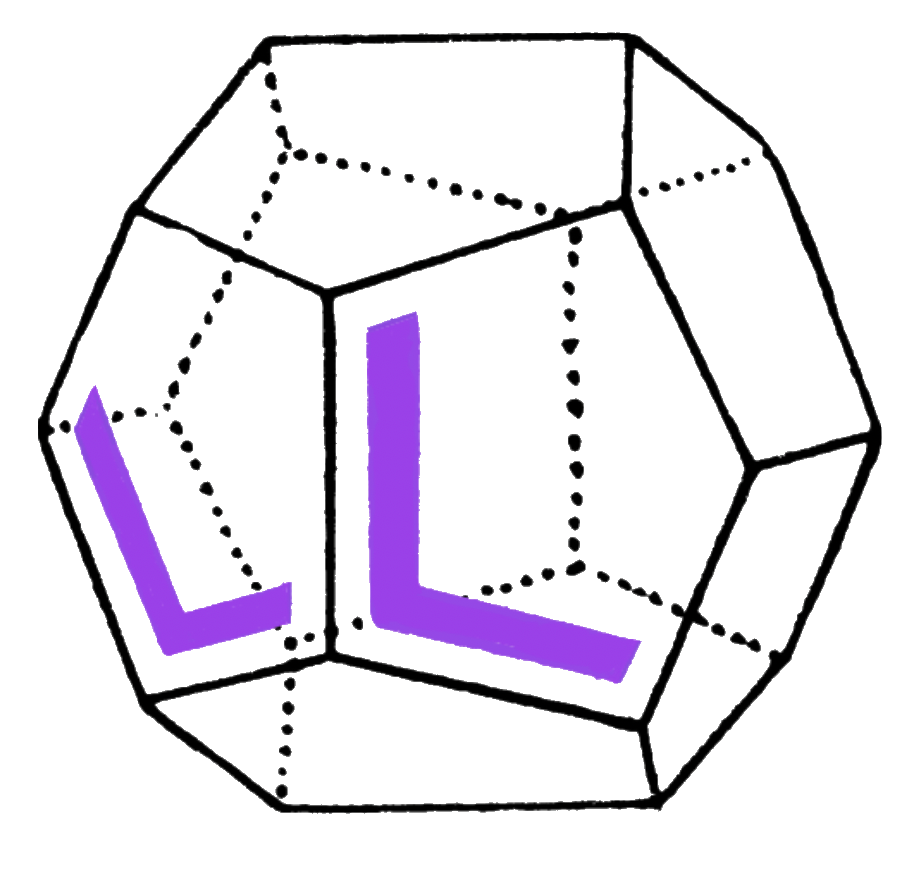
\includegraphics[width=2cm,height=2cm]{ll.png}}

    }}

\AddToShipoutPicture*
  {\put(470,767){
    \href{https://github.com/linlib/CategoriesandHilbertSpaces/StringDiagramGenerator.py}{\texttt{.py file}}
  }}

\AddToShipoutPicture*
  {\put(470,752){
    \href{https://github.com/linlib/TheWhiteheadTheoremandTwoVariations/blob/main/TheWhiteheadTheoremandTwoVariations.tex}{\texttt{.tex file}}\\

  }}


\AddToShipoutPicture*
  {\put(470,737){

    \href{https://github.com/linlib/TheWhiteheadTheoremandTwoVariations/blob/main/TheWhiteheadTheoremandTwoVariations.pdf}{\texttt{.pdf file}}\\

  }}

  \AddToShipoutPicture*
  {\put(470,722){
    \href{https://github.com/linlib/TheWhiteheadTheoremandTwoVariations/blob/main/TheWhiteheadTheoremandTwoVariations.lean}{\texttt{.lean file}}

  }}

\ \\

%LEAN: 
\begin{center}
\begin{tcolorbox}[width=5.8in,colback={white},coltitle=white]
\begin{center}
\ \\
\scalebox{3}{\texttt{The Whitehead Theorem}}\\
\ \\
\scalebox{3}{\texttt{and}}\\
\ \\
\scalebox{3}{\texttt{Two Variations}}\\
\ \\
\end{center}
\end{tcolorbox}
\end{center}
\ \\


\ \\
%LEAN: 
\begin{center}
\begin{tcolorbox}[width=6in,colback={white}]
\begin{center}
\scalebox{0.85}{∀(C:D(∞-Cat)),∀(D:D(∞-Cat)),∀(F:C ⭢ D),∀(G:C ⭢ D),(∀(n:Nat),(π⃗ₙ F = π⃗ₙ G)) → F = G}\\
\ \\
\scalebox{0.85}{∀(X:D(∞-Grpd)),∀(Y:D(∞-Grpd)),∀(f:X ⭢ Y),∀(g:X ⭢ Y),(∀(n:Nat),(π⃡ₙ f = π⃡ₙ g)) → f = g}\\
\ \\
\scalebox{0.85}{∀(X:D(∞-Grpd₀)),∀(Y:D(∞-Grpd₀)),∀(f:X ⭢ Y),∀(g:X ⭢ Y),(∀(n:Nat),(πₙ f = πₙ g)) → f = g}\\
\end{center}
\end{tcolorbox}
\end{center}



\begin{center}
\texttt{Plans to prove three variations of the}\\
\texttt{Whitehead theorem of homotopy groups in}\\
\texttt{Lean 4, with extensive use of Mathlib 4}
\end{center}
\ \\
\ \\


\thispagestyle{empty}


\newpage

\ \\
\ \\

\begin{center}

\pagecolor{white}
\color{black}




\end{center}

\thispagestyle{empty}




\newpage
\pagecolor{white}
\color{black}
\ \\
\ \\
\thispagestyle{empty}
\large %%%%%%%% HERE IS THE large LARGE size textsize set text size
\newpage 
\ \\
\ \\
\ \\
\ \\
\ \\
\ \\
\ \\
\ \\
\ \\
\ \\
\ \\
\thispagestyle{empty}
 
\newpage



\newpage

\ \\
\ \\
\ \\
\ \\
\ \\
\ \\
\ \\
\ \\
\ \\
\ \\
\ \\

We wish to acknowledge the collaborative efforts of E. Dean Young and Jiazhen Xia. Dean Young initially formulated the introduction with twelve goals, posting them on the Lean Zulip in August of 2023. Together the authors are pursuing these plans as a long term project.\\



\newpage



\newpage
\section{Contents}

The table of contents below reflects the tentative long-term goals of the authors, with the main goal the pursuit of the Whitehead theorem for a point-set model involving Mathlib's predefined homotopy groups.\\

{
\footnotesize
\begin{longtable}{|| l || l ||} 
\hline
\multicolumn{1}{||c||}{$\texttt{Section}$} & \multicolumn{1}{|c||}{$\texttt{Description}$} \\
\hline
\hline
Unfinished & \\
\hline
Contents & \\
\hline
Unicode & \\
\hline
Introduction & \\
\hline \hline
\multicolumn{2}{||c||}{\texttt{PART I: } Based Connected ∞-Groupoids} \\
\hline \hline
\multicolumn{2}{||c||}{\texttt{Chapter 1: }Based Connected ∞-Groupoids} \\
\hline \hline
D(∞-Grpd₀) & The derived category of based connected ∞-groupoids \\
\hline
D(∞-Grpd₀/X₀) & The derived category of based connected ∞-groupoids over X₀. \\
\hline
Ω : ∞-Grpd₀ ⭢ ∞-Grpd & The loop space functor \\
\hline
Σ : ∞-Grpd₀ ⭢ ∞-Grpd₀ & The based suspension functor \\
\hline 
ω f : ∞-Grpd/D₀ ⭢ ∞-Grpd/C₀ & The homotopy fiber\\
\hline 
σ f : ∞-Grpd₀/C₀ ⭢ ∞-Grpd₀/D₀ & Based homotopy pushout \\
 \hline 
πₙ : ∞-Grpd₀ ⭢ Set & The connected components functors\\
 \hline \hline
  \multicolumn{2}{||c||}{\texttt{Chapter 2: }The Whitehead Theorem for Based Connected ∞-Groupoids} \\
\hline \hline
Globular Sets & Defining globular sets\\
\hline
HEP for based connected ∞-groupoids & The homotopy extension property for ∞$\texttt{-Grpd}$₀\\
 \hline 
REP for based connected ∞-groupoids & The replacement functor on ∞$\texttt{-Grpd}$₀ \\
\hline
Whitehead theorem (c) & A map $\texttt{F : D(}$∞$\texttt{-Grpd₀).Hom E₀ B₀}$ is determined by $\texttt{λ(n:Nat),πₙ F}$. \\
\hline \hline
  \multicolumn{2}{||c||}{\texttt{Chapter 3: }The Category of Pairs} \\
\hline \hline
HEP for pairs of based connected ∞-groupoids & The homotopy extension property for ∞$\texttt{-Grpd}$₀\\
 \hline 
REP for pairs of based connected ∞-groupoids & The replacement functor on ∞$\texttt{-Grpd}$₀ \\
\hline
The Whitehead theorem for pairs & ... \\
\hline \hline
 \multicolumn{2}{||c||}{\texttt{Chapter 4: }Internal and Operadic Groups} \\
\hline \hline
 $\texttt{InternalGroup}$   & The category of internal groups in Γ  \\
 \hline
 $\texttt{InternalGroupAction G₀}$ & The category of internal G₀-actions in Γ   \\
 \hline
  $\texttt{OperadicGroup}$  & The category of operadic groups  \\
 \hline
 $\texttt{OperadicGroupAction}$  & The category of operadic group actions  \\
 \hline
  The $\texttt{P}$ and $\texttt{O}$ Functors & $\texttt{P = ? • O}$ \\
 \hline
 The $\texttt{p}$ and $\texttt{o}$ Functors & $\texttt{p = ? • o}$ \\
\hline \hline
\multicolumn{2}{||c||}{\texttt{PART II: } ∞-Groupoids} \\
\hline \hline 
\multicolumn{2}{||c||}{\texttt{Chapter 5: }∞\texttt{-Grpd}}\\
\hline \hline
D(∞-Grpd) & The derived category of ∞-groupoids \\
\hline
D(∞-Grpd/X) & The derived category of ∞-groupoids over X \\
\hline
Ω⃡ : ∞-Grpd ⭢ ∞-Grpd & The directed path space functor \\
 \hline 
Σ⃡ : ∞-Grpd ⭢ ∞-Grpd & The unbased suspension functor \\
 \hline 
ω⃡ f : ∞-Grpd⁄D ⭢ ∞-Grpd/C & The directed homotopy pullback functor\\
\hline 
σ⃡ f : ∞-Grpd/C ⭢ ∞-Grpd/D & Homotopy pushout with a point \\
 \hline 
π⃡ₙ : ∞-Grpd ⭢ Set & The connected components functors\\
 \hline \hline
 \multicolumn{2}{||c||}{\texttt{Chapter 6: }The Whitehead Theorem for ∞-Groupoids} \\
\hline \hline
Cubical Complexes & ...\\
\hline
REP for ∞-groupoids & The cofibrant replacement functor for ∞-groupoids\\
\hline
HEP for ∞-groupoids & The homotopy extension property\\
\hline
Whitehead theorem (b) & A map $\texttt{F : D(}$∞$\texttt{-Grpd).Hom E B}$ is determined by $\texttt{λ(n:Nat),}$π⃡ₙ
$\texttt{F}$. \\
\hline \hline
\multicolumn{2}{||c||}{\texttt{Chapter 7: }The Category of Pairs of ∞-Groupoids} \\
\hline \hline
... & ...\\
\hline
REP for pairs of ∞-groupoids & The replacement functor on ∞$\texttt{-Grpd}$ \\
\hline
HEP for pairs of ∞-groupoids & The homotopy extension property for ∞$\texttt{-Grpd}$\\
 \hline 
The Whitehead theorem for pairs of ∞-groupoids & ... \\
\hline \hline
\multicolumn{2}{||c||}{\texttt{Chapter 8: }Internal and Operadic Groupoids and their Actions} \\
\hline \hline
 $\texttt{InternalGroupoid Γ}$   & The category of internal groupoids in Γ \\
 \hline
 $\texttt{InternalGroupoidAction Γ G}$ & The category of internal G-actions in Γ \\
 \hline
  $\texttt{OperadicGroupoid Γ}$  & The category of operadic groupoids  \\
 \hline
 $\texttt{OperadicGroupoidAction Γ}$  & The category of operadic groupoid actions  \\
  \hline
  The $\texttt{P⃡}$ and $\texttt{O⃡}$ Functors & $\texttt{P⃡ = ? • O⃡}$ \\
 \hline
 The $\texttt{p⃡}$ and $\texttt{o⃡}$ Functors & $\texttt{p⃡ = ? • o⃡}$ \\
 \hline \hline
 \multicolumn{2}{||c||}{\texttt{PART III: } ∞-Categories} \\
\hline \hline
\multicolumn{2}{||c||}{\texttt{Chapter 9: }∞\texttt{-Cat}} \\
\hline \hline
D(∞-Cat) & The derived category of ∞-categories \\
\hline
D(∞-Cat⁄C) & The derived category of ∞-categories over C \\
\hline
Ω⃗ : ∞-Cat ⭢ ∞-Cat & The directed path space functor \\
 \hline 
 Σ⃗ : ∞-Cat ⭢ ∞-Cat & The directed unbased suspension \\
\hline 
ω⃗ f : ∞-Cat⁄D ⭢ ∞-Cat/C & The directed homotopy pullback functor\\
 \hline 
 σ⃗ f : ∞-Cat/C ⭢ ∞-Cat/D & The directed homotopy pushout \\
 \hline 
π⃗ₙ : ∞-Cat ⭢ Set & The connected components functors\\
 \hline \hline
 \multicolumn{2}{||c||}{\texttt{Chapter 10: }The Whitehead Theorem for ∞-Categories} \\
\hline \hline
Directed Cubical Complexes & ...\\
\hline
REP for ∞-categories & The cofibrant replacement functor for ∞-categories\\
\hline
HEP for ∞-categories & The directed homotopy extension property\\
\hline 
Whitehead theorem (a) & A map $\texttt{F : D(}$∞$\texttt{-Cat).Hom E B)}$ is determined by $\texttt{λ(n:Nat),}$π⃗ₙ$\texttt{F}$.\\
\hline \hline
\multicolumn{2}{||c||}{\texttt{Chapter 11: }The Category of Pairs of ∞-Categories} \\
\hline \hline
REP for pairs of ∞-groupoids & The replacement functor on ∞$\texttt{-Grpd}$ \\
\hline
HEP for pairs of ∞-groupoids & The homotopy extension property for ∞$\texttt{-Grpd}$\\
 \hline 
The Whitehead theorem for pairs of ∞-groupoids & ... \\
\hline \hline
\multicolumn{2}{||c||}{\texttt{Chapter 12: Internal and Operadic Categories and their Sheaves}} \\
\hline \hline
 $\texttt{InternalCategory : ???}$   & The category of internal categories \\
 \hline
 $\texttt{InternalPresheaf : ???}$  & The category of internal presheaves \\
 \hline
  $\texttt{OperadicCategory : Cat → Cat}$  & The category of operadic categories  \\
 \hline
 $\texttt{OperadicPresheaf : Cat → Cat}$   & The category of operadic presheaves  \\
  \hline
  The $\texttt{P⃗}$ and $\texttt{O⃗}$ Functors & $\texttt{P⃗ = ? • O⃗}$ \\
 \hline
 The $\texttt{p⃗}$ and $\texttt{o⃗}$ Functors & $\texttt{p⃗ = ? • o⃗}$ \\
 \hline
\end{longtable}
}



\newpage
\section{Introduction}

{\bf The main goal of this repository is to prove the Whitehead theorem in Lean 4 using Mathlib 4's homotopy groups}. Two other subsequent goals are to state and prove two variations of the Whitehead theorem. It is important that initial pull requests stemming from our work remain basic and accessible; we hope to make progress which is gradual and incremental.\\

Besides this goal, we have two others. Here are the three Whitehead Theorems which form our main three goals:

\begin{enumerate}[(a)]
\item (The Whitehead theorem) ∀(E:D(∞-Grpd₀)),∀(B:D(∞-Grpd₀)),∀(F:E ⭢ B),∀(G:E ⭢ B),(∀(n:Nat),(πₙ F = πₙ G)) → F = G, where πₙ is notation for π n.
\item (The Whitehead theorem for ∞-groupoids) ∀(E:D(∞-Grpd)),∀(B:D(∞-Grpd)),∀(F:E ⭢ B),∀(G:E ⭢ B),(∀(n:Nat),(π⃡ₙ F = π⃡ₙ G)) → F = G, where π⃡ₙ is notation for π⃡ n.
\item (The Whitehead theorem for ∞-categories) ∀(E:D(∞-Cat)),∀(B:D(∞-Cat)),∀(F:E ⭢ B),∀(G:E ⭢ B),(∀(n:Nat),(π⃗ₙ F = π⃗ₙ G)) → F = G, where π⃗ₙ is notation for π⃗ n.
\end{enumerate}

Here are a few comments on these theorems:
\begin{enumerate}
\item The first Whitehead theorem reflects the known one, which dates back to a paper that can be found in defined on Mathlib 4's homotopy groups, which make use of cubes Iⁿ and their boundaries ∂Iⁿ. There is also a fourth Whitehead theorem concerning ∞-Cat₀, but which is ommited; it is less general than the third while the first is present for its use of Mathlib 4's predefined πₙ's.
\item The unicode symbol ⭢ (U+2B62) reflects a notation not present in Mathlib 4, and which we will make local or scoped.
\item The three theorems above are stated in an order reversed from the order of their implementation.
\end{enumerate}

We will use two models of each of the following categories in the theorems above:

\begin{enumerate}[(i)]
\item We model ∞-Cat : Cat firstly as the category of categories enriched over Mathlib 4's topological spaces, and secondly as the category of quasicategories.
\item We model ∞-Grpd : Cat firstly as a Mathlib 4's topological spaces, and secondly as the category of Kan complexes.
\item We model ∞-Grpd₀ : Cat firstly as the based connected objects using Mathlib 4's topological spaces, and secondly as the category of based connected Kan complexes.
\end{enumerate}

This choice accords with the standard approach to the third theorem, in which one typically chooses both a combinatorial and point-set model, with the former featuring a \href{https://github.com/leanprover-community/mathlib4/blob/8666bd82efec40b8b3a5abca02dc9b24bbdf2652/Mathlib/AlgebraicTopology/SimplicialSet.lean#L235-L236}{geometric realization functor} into the latter.\\

We will make heavy use of $\texttt{Mathlib 4}$'s material on category theory, particularly their categories, functors, and natural transformations:

\begin{enumerate}
\item Categories (see Mathlib's $\texttt{Category X}$)
\item Functors (see Mathlib's $\texttt{Functor C D}$)
\item Natural transformations (see Mathlib's $\texttt{NatTrans F G}$)
\item Equations between natural transformations (see Mathlib's $\texttt{NatExt}$ here; these are related to our $\texttt{equation}$)
\end{enumerate}

While the functors πₙ occuring in the main theorems above are already defined in $\texttt{Mathlib}$ for the desired point-set model, the functors π⃗ₙ and π⃡ₙ are not, and their definition will require great care. Here are their types:

\begin{enumerate}[(i)]
\item π⃗ₙ : Functor ∞-Cat Set
\item π⃡ₙ : Functor ∞-Grpd Set
\item πₙ : Functor ∞-Grpd₀ Set
\end{enumerate}

We may wish to modify these types out of convenience and to accord with the pre-existing functors πₙ in $\texttt{Mathlib 4}$.\\

The existence of a base point makes πₙ relatively straightforward to define, while π⃗ₙ and π⃡ₙ `grow' as n does. We also form their derived functors:

\begin{enumerate}[(i)]
\item D(π⃗ₙ) : D(∞-Cat) ⭢ D(Set) ≃ Set
\item D(π⃡ₙ) : D(∞-Grpd) ⭢ D(Set) ≃ Set
\item D(πₙ) : D(∞-Grpd₀) ⭢ D(Set) ≃ Set
\end{enumerate}

In the course of the repository we will need the directed path space, path space, and loop space functors as well, which fit with the analogy formed by the Whitehead theorem and its two variations:

\begin{enumerate}
\item Ω⃗ : ∞-Cat ⭢ ∞-Cat sends \iffalse C to a [(Sⁿ⁻¹,Dⁿ),(C,C)]\fi
\item Ω⃡ : ∞-Grpd ⭢ ∞-Grpd is ...
\item Ω is the loop space functor
\end{enumerate}

\iffalse
The choice of ∞-Cat\_(A) as a model is complementary to our discussion of operadic structures. In this 
\fi

We develop two models of (∞,1)-categories, one combinatorial in nature and another point-set in nature. 

\iffalse
The latter, developed first, features a deformation retraction γ⃗ $\leftrightarrow$ γ⃗² between the directed unit interval and its cartesian product with itself.\\
\fi

The third theorem (c), is the one from Whitehead's original papers.\\

With the choice of quasicategories as a combinatorial model, we hope to give good integration with Mathlib's existing features (though technically only the inner horns and simplices are defined, not even the category of quasicategories itself).\\

In the directed context, a homotopy between two maps in ∞-Cat⁄C consists of a sequence of compatible directed homotopies with the odd morphisms in the sequence formed from reversed copies of Δ¹. Really we have two such categories, one of which consists of formal words, and another which involves ∞-categories and ∞-functors in the image of $\texttt{repl}$).\\

The main technical feature in the proofs of these theorems concerns a lifting property which successively lifts a homotopy along a single attachment of Δⁿ along its boundary ∂Δⁿ. A homotopy h : ∂Δⁿ × Δ¹ ⭢ Y between f, g : ∂Δⁿ ⭢ Y extends to a map H : Δⁿ × Δ¹ ⭢ Y. The directed case requires an extra technical feature. H(-,1) and g match on ∂Δⁿ, producing a map f : X ⭢ Y, where X consists of two copies of Δⁿ glued together at the boundary.\\

Consider a space X' formed as a quotient of Δⁿ × Δ¹ by ∂Δⁿ × Δ¹. There is a map φ : X ⭢ X'. An induction hypothesis on f and g involving πₙ ensures that the aparent map X ⭢ Y lifts along φ, producing a map from Δⁿ × Δ¹ which is constant on ∂Δⁿ × Δ¹. Stacking this on top of H can be done using an isomorphism between Δ¹ and Δ¹ glued with itself along different endpoints. Altogether this produces a homotopy between f and g.\\

We will define three different kinds of derived category:\\

\begin{enumerate}
\item D(∞-Cat) : Cat (the directed derived category of ∞-categories)
\item D(∞-Grpd) : Cat (the derived category of ∞-groupoids)
\item D(∞-Grpd₀) : Cat (the derived category of based ∞-groupoids)
\end{enumerate}

We then create the second kind of derived category, one for each of the objects in the respective categories above:

\begin{enumerate}
\item For C : D(∞-Cat), a category D(∞-Cat/C) : Cat
\item For G : D(∞-Grpd), a category D(∞-Grpd/G) : Cat
\item For G₀ : D(∞-Grpd₀), a category D(∞-Grpd₀/G₀) : Cat
\end{enumerate}

For the model built on simplicial sets, Ω⃗ will be representable by Δ¹ with respect to an internal hom, and Ω⃡ will be representable by a model of the unit interval I := [0,1].\\

We will use six (strict) ``internal'' structures in addition to the standard structures in category theory:

\begin{enumerate}[(i)]
\item InternalCategory : Cat → Cat 
\item InternalPresheaf : (X : Cat) → (C : (InternalCategory X)) → Cat
\item InternalGroupoid : Cat → Cat
\item InternalGroupoidAction : (X : Cat) → (G : (InternalGroupoid X)) → Cat
\item InternalGroup : Cat → Cat
\item InternalGroupAction : (X : Cat) → (G₀ : (InternalGroup X)) → Cat   
\end{enumerate}

The book ``Galois theories" by Borceux and Janelidze contains the internal structures (iii), (iv), (v), and (vi), and the first two internal structures have fewer entries. That book details how to think about Galois theory using internal groupoids, internal G-presheaves, monadicity, comonadicity, and the constructions involved in Eilenberg-Moore theory.\\

Some previous work done on these structures can be found at the thread \href{https://leanprover.zulipchat.com/#narrow/stream/116395-maths/topic/Internal.20categories}{here}.\\

The six internal structures above arise here in relation to six functors:

\begin{enumerate}[(I)]
\item Ω⃗ : ∞-Cat ⭢ ∞-Cat (notation for the directed path space functor, related to [Δ¹,-]). D(Ω⃗) factors through internal categories in D(∞-Cat) by a categorical equivalence D(∞-Cat) ≅ InternalCategory D(∞-Cat) (internal categories in D(∞-Cat))
\item ω⃗ (𝟙 C) : ∞-Cat/C ⭢ ∞-Cat/C, the derived directed homotopy pullback with 𝟙 C. D(ω⃗ (𝟙 C)) factors through a categorical equivalence between D(∞-Cat/C) and internal P⃗C-presheaves in D(∞-Cat/C).
\item Ω⃡ : ∞-Grpd ⭢ ∞-Grpd (notation for the path space functor [I,-]), the derived homotopy pullback of an ∞-groupoid with itself. D(Ω⃡) factors through a categorical equivalence between D(∞-Grpd) and internal groupoids in D(∞-Grpd)
\item ω⃡ (𝟙 X) : ∞-Grpd/X ⭢ ∞-Grpd/X, the derived homotopy pullback with 𝟙 X. D(ω⃡ (𝟙 X)) factors through internal P⃡X
\item Ω : ∞-Grpd₀ ⭢ ∞-Grpd₀, the loop space functor. D(Ω) factors through a categorical equivalence between D(∞-Grpd₀) and internal groups in D(∞-Grpd₀) (the loop space functor on connected based ∞-groupoids)
\item ω (𝟙 X) : ∞-Grpd₀/X₀ ⭢ ∞-Grpd₀/X₀, the homotopy pullback with the base of X₀. D(ω (𝟙 X)) factors through internal PX₀-actions in based connected spaces over X₀.
\end{enumerate}

(v) in the above is shown \href{https://mathoverflow.net/questions/128883/why-omega-x-and-bg-are-adjoint-functors}{here} and (vi) in the above is shown in a typical exposition of $G$-principal bundles.\\

The functors ω⃗ (𝟙 C), ω⃡ (𝟙 X), and ω (𝟙 C) in the above ensue from a more general construction:\\

\begin{enumerate}
\item For C, D : D(∞-Cat), and f : C ⭢ D, ω⃗ f : D(∞-Cat/D) ⭢ D(∞-Cat/C)   (derived directed homotopy pullback)
\item For B, E : D(∞-Grpd), and f : E ⭢ B, ω⃡ f : D(∞-Grpd/B) ⭢ D(∞-Grpd/E) (derived homotopy pullback)
\item For B₀, E₀ : D(∞-Grpd₀), and f : E₀ ⭢ B₀, ω f : D(∞-Grpd₀/B₀) ⭢ D(∞-Grpd₀/E₀) (homotopy pullback with the base)
\end{enumerate}

These six factored functors P⃗ , P⃡ , P : D(∞-Grpd₀), p⃗ (𝟙 C), p⃡ (𝟙 X), p are each fully faithful and produce categorical equivalences; we later construct functors B⃗, B⃡, B, b⃗, b⃡, b defined on the essential image of these six, which are inverse to them up to natural isomorphism.\\

We obtain six categorical equivalences witnessed by these twelve functors (along with twelve natural isomorphisms). Here are the types of P⃗ , P⃡ , P : D(∞-Grpd₀), p⃗ (𝟙 C), p⃡ (𝟙 X), p:

\begin{enumerate}
\item The directed path space, the path space, and loop space form components of the functors P⃗, P⃡, and P, which are valued in internal categories, internal groupoids, and internal groups respectively.
\begin{enumerate}
\item P⃗ : D(∞-Cat) ⭢ Cat D(∞-Cat)
\item P⃡ : D(∞-Grpd) ⭢ Grpd D(∞-Grpd)
\item P : D(∞-Grpd₀) ⭢ Grp D(∞-Grpd) (see \href{https://mathoverflow.net/questions/128883/why-omega-x-and-bg-are-adjoint-functors}{here})
\end{enumerate}
\item The directed homotopy pullback, the homotopy pullback, and the homotopy pullback with the base form components of the functors Alg(Mon(ω⃗)), Alg(Mon(ω⃡)), and Alg(Mon(p)), respectively. 
\begin{enumerate}
\item p⃗ (𝟙 C) : D(∞-Cat⁄C) ⭢ InternalPresheaf D(∞-Cat⁄C) P⃗.obj C 
\item p⃡ (𝟙 X) : D(∞-Grpd⁄X) ⭢ InternalGroupoidAction D(∞-Grpd⁄X) P⃡.obj X
\item p (𝟙 X₀) : D(∞-Grpd₀⁄X₀) ⭢ InternalGroupAction D(∞-Grpd₀⁄X₀) P.obj X₀
\end{enumerate}
\end{enumerate}

Above, the functors P⃗, P⃡, P, p⃗, p⃡, and p feature Ω⃗, Ω⃡, Ω, ω⃗, ω⃡, and ω in their components, and can be related to them using constructions from Eilenberg-Moore theory.\\

\iffalse
Interspersing one of the 6 omegas's in each of six operadic structures, which have the same number of entries as the six internal structures respectively. In the thirteen entry operadic category, one of the entries is an ordinary object in the category, analogous to the first of the thirteen entries of the internal category. The second entry, instead of featuring the ordinal 2 (the morphism component, which is the second of two entries in the category in question), features a sequence of objects in the category. The identity morphism Idn : Obj ⭢ Mor of the internal category with 13 entries (as opposed to the slightly more complex structure in which separate clauses assume the existence of the relevant pullbacks so as to create an endofunction of Cat) is analogous to a function also from O₀ to O₁, and two further entires are essentially shared by both as well: Dom and Cod. One difference occurs in the component of an internal category for the properties that Idn has, which in the operadic case is 
\fi

\iffalse
J : Nat → ∞-Grpd
\fi

\iffalse
Ω⃗, Ω⃡, Ω⃗₀, Ω⃡₀ are the ones I construct and Ω Mathlib's.
\fi

\iffalse
Adding in the operadic structures.
\fi


\iffalse
https://leanprover.zulipchat.com/#narrow/stream/116395-maths/topic/Internal.20categories
\fi

{
\footnotesize
\begin{center}
\begin{tabular}{||l || l || l || l ||} 
 \hline
  \multicolumn{4}{||c||}{\texttt{Twelve Structures}} \\
 \hline
 \multicolumn{2}{||c||}{\texttt{Strict}}  &  \multicolumn{2}{||c||}{\texttt{Lax}} \\
 \hline
 \texttt{Unitial} &  \texttt{Actional}  &  \texttt{Unitial} &  \texttt{Actional}\\
 \hline \hline
 \texttt{InternalCategory}  & \texttt{InternalPresheaf} & \texttt{OperadicCategory} & \texttt{OperadicPresheaf} \\ 
 \hline
 \texttt{InternalGroupoid} & \texttt{InternalGroupoidAction} & \texttt{OperadicGroupoid} & \texttt{OperadicGroupoidAction} \\ 
 \hline
\texttt{InternalGroup} & \texttt{InternalGroupAction} & \texttt{OperadicGroup} & \texttt{OperadicGroupAction} \\ 
 \hline 
\end{tabular}
\end{center}
}
\iffalse
{\footnotesize
\begin{center}
\scalebox{1.1}{
\begin{tabular}{|| l | l || l | l || } 
\hline
\hline
\multicolumn{2}{||c||}{Internal} & \multicolumn{2}{||c||}{Operadic} \\
\hline
\multicolumn{2}{||c||}{Unitial} & \multicolumn{2}{||c||}{Actional} & \multicolumn{2}{||c||}{Unitial} & \multicolumn{2}{||c||}{Actional} \\
\hline
\hline
$\texttt{InternalCategory : Cat → Cat}$ & $\texttt{InternalPresheaf : (C : Cat) → (InternalCategory C) → Cat}$ & $\texttt{OperadicCategory\_(-) : ∞-Cat\_(-) → ∞-Cat\_(-)}$ & OperadicPresheaf\_(-) : (X : ∞-Cat\_(-)) → ∞-Cat\_{(-)} \\
\hline
$\texttt{InternalGroupoid\_(-) : Cat\_(-) → Cat\_(-)}$ & $\texttt{InternalGroupoidAction : (C : Cat) → (InternalGroupoid C) → Cat}$& $\texttt{OperadicGroupoid\_(-) : ∞-Cat\_(-) → ∞-Cat\_(-)}$ & OperadicGroupoidAction\_(-) : (OperadicGroupoid\_() C) → (InternalCategory C) → ∞-Cat\_(-) → ∞-Cat\_(-) \\
\hline
$\texttt{InternalMonoid\_(-) : Cat\_(-) → Cat\_(-)}$ & $\texttt{InternalMonoidAction : (C : Cat) → (InternalMonoid C) → Cat}$ & $\texttt{OperadicMonoid\_(-) : ∞-Cat\_(-) → ∞-Cat\_(-)}$ & $\texttt{OperadicMonoidAction}$\_$\texttt{(-) : ∞-Cat\_(-) → ∞-Cat\_(-)}$\\
\hline
$\texttt{InternalGroup\_(-) : Cat\_(-) → Cat\_(-)}$ & $\texttt{InternalGroupAction : (C : Cat) → (InternalGroup C) → Cat}$ & $\texttt{OperadicGroup\_(-) : ∞-Cat\_(-) → ∞-Cat\_(-)}$ & $\texttt{OperadicGroupAction}$\_$\texttt{(-) : ∞-Cat\_(-) → ∞-Cat\_(-)}$\\
 \hline
\end{tabular}}
\end{center}}
\fi

\ \\
{\footnotesize
\begin{center}
\scalebox{1.1}{
\begin{tabular}{|| l || l ||} 
\hline
\hline
Ω⃗ : ∞-Cat ⭢ ∞-Cat & ω⃗ : (C : ∞-Cat) → (D : ∞-Cat) → (F : ∞-Cat.hom C D) → (∞-Cat⁄D) ⭢ ∞-Cat \\
\hline
O⃗ : ∞-Cat ⭢ OperadicCategory ∞-Cat & o⃗ : (C : ∞-Cat) → (D : ∞-Cat) → (F : ∞-Cat.hom C D) → (∞-Cat⁄D) ⭢ OperadicPresheaf (O⃗.obj D)\\
\hline
P⃗ : ∞-Cat ⭢ InternalCategory D(∞-Cat) & p⃗ : (C : ∞-Cat) → (D : ∞-Cat) → (F : ∞-Cat.hom C D) → (∞-Cat⁄D) ⭢ InternalPresheaf (P⃗.obj D) \\
\hline
\hline
Ω⃡ : ∞-Grpd ⭢ ∞-Grpd & ω⃡ : (X : ∞-Grpd) → (Y : ∞-Grpd) → (F : ∞-Cat.hom X Y) → (∞-Grpd⁄Y) ⭢ ∞-Grpd \\
\hline
O⃡ : ∞-Grpd ⭢ OperadicGroupoid ∞-Grpd & o⃡ : (X : ∞-Grpd) → (Y : ∞-Grpd) → (F : ∞-Cat.hom X Y) → (∞-Grpd⁄Y) ⭢ OperadicGroupoidAction (O⃡.obj Y) \\
\hline
P⃡ : ∞-Grpd ⭢ InternalGroupoid D(∞-Grpd) & p⃡ : (X : ∞-Grpd) → (Y : ∞-Grpd) → (F : ∞-Cat.hom C D) → (∞-Grpd⁄Y) ⭢ InternalGroupoidAction (P⃡.obj Y)  \\
\hline
\hline
Ω : ∞-Grpd₋₁ ⭢ ∞-Grpd₋₁  & ω : (X₋₁ : ∞-Grpd₋₁) → (Y₋₁ : ∞-Grpd₋₁) → (F : ∞-Grpd₋₁.hom X₋₁ Y₋₁) → (∞-Grpd₋₁⁄Y₋₁) ⭢ ∞-Grpd₋₁ \\
\hline
O : ∞-Grpd₋₁ ⭢ OperadicGroup ∞-Grpd₋₁ & o : (X₋₁ : ∞-Grpd₋₁) → (Y₋₁ : ∞-Grpd₋₁) → (F : ∞-Grpd₋₁.hom X₋₁ Y₋₁) → (∞-Grpd₋₁⁄Y₋₁) ⭢ OperadicGroupAction (O.obj X) \\
\hline
P : ∞-Grpd₋₁ ⭢ InternalGroup D(∞-Grpd₋₁) & p : (X₋₁ : ∞-Grpd₋₁) → (Y₋₁ : ∞-Grpd₋₁) → (F : ∞-Grpd₋₁.hom X₋₁ Y₋₁) → (∞-Grpd₋₁⁄Y₋₁) ⭢ InternalGroupAction (P.obj X₋₁) \\
\hline
 \hline
\end{tabular}}
\end{center}}




\iffalse
░▒▓█▓▒░░▒▓█▓▒░▒▓███████▓▒░░▒▓█▓▒░░▒▓██████▓▒░ ░▒▓██████▓▒░░▒▓███████▓▒░░▒▓████████▓▒░ 
░▒▓█▓▒░░▒▓█▓▒░▒▓█▓▒░░▒▓█▓▒░▒▓█▓▒░▒▓█▓▒░░▒▓█▓▒░▒▓█▓▒░░▒▓█▓▒░▒▓█▓▒░░▒▓█▓▒░▒▓█▓▒░        
░▒▓█▓▒░░▒▓█▓▒░▒▓█▓▒░░▒▓█▓▒░▒▓█▓▒░▒▓█▓▒░      ░▒▓█▓▒░░▒▓█▓▒░▒▓█▓▒░░▒▓█▓▒░▒▓█▓▒░        
░▒▓█▓▒░░▒▓█▓▒░▒▓█▓▒░░▒▓█▓▒░▒▓█▓▒░▒▓█▓▒░      ░▒▓█▓▒░░▒▓█▓▒░▒▓█▓▒░░▒▓█▓▒░▒▓██████▓▒░   
░▒▓█▓▒░░▒▓█▓▒░▒▓█▓▒░░▒▓█▓▒░▒▓█▓▒░▒▓█▓▒░      ░▒▓█▓▒░░▒▓█▓▒░▒▓█▓▒░░▒▓█▓▒░▒▓█▓▒░        
░▒▓█▓▒░░▒▓█▓▒░▒▓█▓▒░░▒▓█▓▒░▒▓█▓▒░▒▓█▓▒░░▒▓█▓▒░▒▓█▓▒░░▒▓█▓▒░▒▓█▓▒░░▒▓█▓▒░▒▓█▓▒░        
 ░▒▓██████▓▒░░▒▓█▓▒░░▒▓█▓▒░▒▓█▓▒░░▒▓██████▓▒░ ░▒▓██████▓▒░░▒▓███████▓▒░░▒▓████████▓▒░
\fi
\newpage
\section{Unicode}

Here is a list of the unicode characters we will use:

{\footnotesize
\begin{center}
\begin{tabular}{|| l || l || l || l ||} 
\hline
$\texttt{Symbol}$ & $\texttt{Unicode}$ & \texttt{VSCode shortcut} & $\texttt{Use}$\\
\hline
\hline
\multicolumn{4}{||c||}{\texttt{Lean's Kernel}} \\
\hline
\hline
× & 2A2F & \backslash\texttt{times} & Product of types\\
\hline
→ & 2192 & \backslash\texttt{rightarrow}  & Hom of types\\
\hline
⟨,⟩ & 27E8,27E9 & \backslash\texttt{langle},\backslash\texttt{rangle}  & Product term introduction\\
\hline
↦ & 21A6 &\backslash\texttt{mapsto}  & Hom term introduction\\
\hline
∧ & 2227 &\backslash\texttt{wedge}  & Conjunction \\
\hline
∨ & 2228 &\backslash\texttt{vee}  & Disjunction \\
\hline
∀ & 2200 &\backslash\texttt{forall}  & Universal quantification \\
\hline
∃ & 2203 &\backslash\texttt{exists}  & Existential quantification\\
\hline
¬ & 00AC &\backslash\texttt{neg}  & Negation\\
\hline
\hline
\multicolumn{4}{||c||}{\texttt{Variables and Constants}} \\
\hline
\hline
ᵃ,ᵇ,ᶜ,...,ᶻ & 1D52,1D56 & & Variables and constants \\
\hline
⁰,¹,²,³,⁴,⁵,⁶,⁷,⁸,⁹ & 1D52,1D56 &  & Variables and constants \\
\hline
⁻ & 207B &  & Variables and constants \\
\hline
₀,₁,₂,₃,₄,₅,₆,₇,₈,₉ & 2080 - 2089 & \backslash\texttt{0}-\backslash\texttt{9} & Variables and constants\\
\hline
𝔸,...,ℤ & 1D538 &  &  \\
\hline
𝕒,...,𝕫 & 1D552 &  &  \\
\hline
𝐀,...,𝐙 & 1D41A &  &  \\
\hline
𝐚,...,𝐳 & 1D41A &  &  \\
\hline
\texttt{α}-\texttt{ω},\texttt{A}-\texttt{Ω} & 03B1-03C9 & & Variables and constants\\
\hline
\hline
\multicolumn{4}{||c||}{\texttt{Categories}} \\
\hline
\hline
 𝟙 & 1D7D9 & \backslash\texttt{b1}  & The identity morphism\\
\hline
 ∘ & 2218 & \backslash\texttt{circ}  & Composition\\
 \hline
 \hline
 \multicolumn{4}{||c||}{\texttt{Bicategories}} \\
 \hline 
 \hline
 • & 2022  & \backslash\texttt{smul}  & Horizontal composition of objects\\ 
  \hline
  \hline
 \multicolumn{4}{||c||}{\texttt{Adjunctions}} \\
\hline
\hline
⇄ & 21C4 & \backslash\texttt{rightleftarrows}  & Adjunctions \\
\hline
⇆ & 21C6 & \backslash\texttt{leftrightarrows}  & Adjunctions \\
\hline
𛲔 & 1BC94 &  & Right adjoints\\
\hline
ॱ & 0971 &  & Left adjoints \\
\hline
⊣ & 22A3 & \backslash\texttt{dashv}  & The condition that two functors are adjoint \\
\hline
\hline
\multicolumn{4}{||c||}{\texttt{Monads and Comonads}} \\
\hline
\hline
?,¿ & 003F, 00BF & ?,\backslash\texttt{?}  & The corresponding (co)monad of an adjunction\\
\hline
!,¡ & 0021, 00A1 & !, \backslash\texttt{!}  & The (co)-Eilenberg-(co)-Moore adjunction \\
\hline
ꜝ,ꜞ & A71D, A71E &  & The (co)exponential maps\\
\hline
\hline
\multicolumn{4}{||c||}{\texttt{Miscellaneous}} \\
\hline
\hline
∼ & 223C & \backslash\texttt{sim} & Homotopies \\
\hline
≃ & 2243 & \backslash\texttt{equiv}  & Equivalences \\
\hline
≅ & 2245 & \backslash\texttt{cong}  & Isomorphisms \\
\hline
⊥ & 22A5 & \backslash\texttt{bot}  & The overobject classifier \\
\hline
∞ & 221E & \backslash\texttt{infty}  & Infinity categories and infinity groupoids\\ 
\hline
${}^{\leftrightarrow}$ & 20D7 &  & Homotopical operations on ∞-categories \\
\hline
${}^{\rightarrow}$ & 20E1 &  & Homotopical operations on ∞-groupoids \\
\hline
\end{tabular}
\end{center}}

Of these, the characters $\texttt{ꜝ,ꜞ,𛲔,ॱ}$,${}^{\rightarrow}$, and ${}^{\leftrightarrow}$ do not have VSCode shortcuts.\\

\ \\
\ \\
\ \\

\iffalse
o⃗ : (C : ∞-Cat) → ∞-Cat⁄C ⭢ OperadicPresheaf (O⃗.obj C)
o⃡ : (X : ∞-Grpd) → ∞-Grpd⁄X ⭢ OperadicGroupoidAction (O⃡.obj X)
o : (X₀ : ∞-Grpd₀) → ∞-Grpd₀⁄X₀ ⭢ OperadicGroupAction (O.obj X₀)
\fi

\newpage
\section{Introduction to \texttt{Lean 4}}

The main way to tell Lean 4 what something means is with $\texttt{def}$, which defines a term in \href{https://leanprover.github.io/theorem_proving_in_lean/dependent_type_theory.html}{dependent type theory}. Much in the same way as other computer languages, we then supply the type of the term (e.g. $\texttt{Int}$ for integer), followed by the formula itself:

%LEAN: 
\begin{center}
\begin{tcolorbox}[width=5in,colback={white},title={\begin{center}\texttt{Lean \thelcounter} \addtocounter{lcounter}{1}  \end{center}},colbacktitle=Blue,coltitle=black]
\begin{minted}[breaklines, escapeinside=||||]{lean}

def zero : Nat := 0

\end{minted}
\end{tcolorbox}
\end{center}

Here we have introduced a natural number $\texttt{n}$ using the type $\texttt{Nat}$ that comes with Lean 4.\\

As a beginner, it's normal to take some time to get comfortable with Lean and formal proof systems. It's a journey that requires practice and patience. Lean has an \href{https://leanprover.zulipchat.com}{active community} that provides support and resources to help you along the way.\\

Constituents of $\texttt{x, y : X}$ of types $\texttt{X}$ can also stand to be equal or unequal, written $\texttt{x = y}$, and it is the properties of equality which in addition to the dependent type theory make a type behave like a set. Equality satisfies the three properties of an equivalence relation, which we cover presently. Consider first the reflexivity property of equality:\\

%LEAN: 
\begin{center}
\begin{tcolorbox}[width=5in,colback={white},title={\begin{center}\texttt{Lean \thelcounter} \addtocounter{lcounter}{1}  \end{center}},colbacktitle=Blue,coltitle=black]
\begin{minted}[breaklines, escapeinside=||||]{lean}

def reflexivity {X : Type} {x : X} : x = x := Eq.refl x

\end{minted}
\end{tcolorbox}
\end{center}

This command defines a function called reflexivity that proves the reflexivity property of equality. The function takes two type parameters: $\texttt{X}$ represents the type of the elements being compared, and $\texttt{x}$ represents an element of type $\texttt{X}$. It also takes an argument ω which is a proof that $\texttt{x}$ is equal to itself ($\texttt{x = x}$). The function body states that the result of $\texttt{reflexivity}$ is the proof ω itself using the $\texttt{Eq.refl}$ constructor, which indicates that $\texttt{x}$  is equal to itself.

In $\texttt{Lean 4}$, $\{\texttt{x : X}\}$ represents an implicit argument, where Lean will attempt to infer the value of $\texttt{x}$ based on the context. $\texttt{(x : X)}$ represents an explicit argument, requiring the value of $\texttt{x}$ to be provided explicitly when using the function or definition.

%LEAN: 
\begin{center}
\begin{tcolorbox}[width=5in,colback={white},title={\begin{center}\texttt{Lean \thelcounter} \addtocounter{lcounter}{1}  \end{center}},colbacktitle=Blue,coltitle=black]
\begin{minted}[breaklines, escapeinside=||||]{lean}

def symmetry {X : Type} {x : X} {y : X}  (p : x = y) := Eq.symm p

\end{minted}
\end{tcolorbox}
\end{center}

This command defines a function called symmetry that proves the symmetry property of equality. It takes three type parameters: $\texttt{X}$ represents the type of the elements being compared, and $\texttt{x}$ and $\texttt{y}$ represent elements of type $\texttt{X}$. The function also takes an argument ω which is a proof that $\texttt{x}$ is equal to $\texttt{y}$ ($\texttt{x=y}$). The function body states that the result of $\texttt{symmetry}$ is the proof ω itself using the $\texttt{Eq.symm}$ constructor, which allows you to reverse an equality proof.

%LEAN: 
\begin{center}
\begin{tcolorbox}[width=5in,colback={white},title={\begin{center}\texttt{Lean \thelcounter} \addtocounter{lcounter}{1}  \end{center}},colbacktitle=Blue,coltitle=black]
\begin{minted}[breaklines, escapeinside=||||]{lean}

def transitivity {X : Type} {x : X} {y : X} {z : X} (p : x = y) (q : y = z) := Eq.trans p q

\end{minted}
\end{tcolorbox}
\end{center}

This command defines a function called transitivity that proves the transitivity property of equality. It takes four type parameters: $\texttt{X}$ represents the type of the elements being compared, and $\texttt{x}$, $\texttt{y}$, and $\texttt{z}$ represent elements of type $\texttt{X}$. The function also takes two arguments $\texttt{p}$ and $\texttt{q}$. $\texttt{p}$ is a proof that $\texttt{x}$ is equal to $\texttt{y}$ ($\texttt{x = y}$), and $\texttt{q}$ is a proof that $\texttt{y}$ is equal to $\texttt{z}$ ($\texttt{y = z}$). The function body states that the result of transitivity is the proof of the composition of ω and $\texttt{q}$ using the $\texttt{Eq.trans}$ constructor, which allows you to combine two equality proofs to obtain a new one.\\

These $\texttt{Lean}$ commands define functions that prove fundamental properties of equality: reflexivity (every element is equal to itself), symmetry (equality is symmetric), and transitivity (equality is transitive). These properties are essential for reasoning about equality in mathematics and formal proofs.\\

We must also require that functions satisfy extensionality:

%LEAN: some essential features of equality
\begin{center}
\begin{tcolorbox}[width=5in,colback={white},title={\begin{center}\texttt{Lean \thelcounter} \addtocounter{lcounter}{1}  \end{center}},colbacktitle=Blue,coltitle=black]
\begin{minted}[breaklines, escapeinside=||||]{lean}

def extensionality (f g : X → Y) (p : (x:X) → f x = g x) : f = g := funext p

\end{minted}
\end{tcolorbox}
\end{center}

Extensionality, a key characteristic of sets and types, asserts that functions which are equal on all values are themselves equal, and it is featured prominently in what is perhaps the most well known mathematical foundations of \href{https://encyclopediaofmath.org/wiki/ZFC}{ZFC}.\\

There are several other features of equality with respect to functions which we should be aware of:

%LEAN: 
\begin{center}
\begin{tcolorbox}[width=5in,colback={white},title={\begin{center}\texttt{Lean \thelcounter} \addtocounter{lcounter}{1}  \end{center}},colbacktitle=Blue,coltitle=black]
\begin{minted}[breaklines, escapeinside=||||]{lean}

def equal_arguments {X : Type} {Y : Type} {a : X} {b : X} (f : X → Y) (p : a = b) : f a = f b := congrArg f p

def equal_functions {X : Type} {Y : Type} {f₁ : X → Y} {f₂ : X → Y} (p : f₁ = f₂) (x : X) : f₁ x = f₂ x := congrFun ω x

def pairwise {A : Type} {B : Type} (a₁ : A) (a₂ : A) (b₁ : B) (b₂ : B) (p : a₁ = a₂) (q : b₁ = b₂) : (a₁,b₁)=(a₂,b₂) := (congr ((congrArg Prod.mk) p) q)

\end{minted}
\end{tcolorbox}
\end{center}

Here are some introductions to Lean 4 and Mathlib 4:

\begin{enumerate}
\item The tutorial \href{https://leanprover.github.io/theorem_proving_in_lean4/}{here} gives an introduction to using the dependent type theory in Lean.
\item 
\end{enumerate}


\part{BASED CONNECTED ∞-GROUPOIDS}

In this first section we prove the standard Whitehead theorem.\\


\chapter{Chapter 1: ∞\texttt{-Grpd₀}}


\noindent\textcolor{Red}{\rule{16cm}{1mm}}
\begin{center}
\texttt{Implementation Progress}
\end{center}
\noindent\textcolor{Red}{\rule{16cm}{1mm}}


%LEAN: CWComplex
\begin{center}
\begin{tcolorbox}[width=5in,colback={white},title={\begin{center}\texttt{Lean \thelcounter} \addtocounter{lcounter}{1}  \end{center}},colbacktitle=Blue,coltitle=black]
\begin{minted}[breaklines, escapeinside=||||]{lean}

/-- A relative CW-complex contains an expanding sequence of subspaces `sk i`
(called the `i`-skeleta) for `i ≥ -1`, where `sk (-1)` is an arbitrary topological space,
isomorphic to `A`, and each `sk (n+1)` is obtained from `sk n` by attaching (n+1)-disks. -/
structure RelativeCWComplex (A : TopCat) where
  /-- Skeleta -/
  sk : ℤ → TopCat
  /-- A is isomorphic to the (-1)-skeleton. -/
  iso_sk_neg_one : A ≅ sk (-1)
  /-- The (n+1)-skeleton is obtained from the n-skeleton by attaching (n+1)-disks. -/
  attach_cells : (n : ℤ) → CWComplex.AttachCells (sk n) (sk (n + 1)) n

/-- A CW-complex is a relative CW-complex whose (-1)-skeleton is empty. -/
abbrev CWComplex := RelativeCWComplex (TopCat.of Empty)

\end{minted}
\end{tcolorbox}
\end{center}

%LEAN: CWComplexCat (topology)
\begin{center}
\begin{tcolorbox}[width=5in,colback={white},title={\begin{center}\texttt{Lean \thelcounter} \addtocounter{lcounter}{1}  \end{center}},colbacktitle=Blue,coltitle=black]
\begin{minted}[breaklines, escapeinside=||||]{lean}

/-- The topology on a relative CW-complex -/
def toTopCat {A : TopCat} (X : RelativeCWComplex A) : TopCat :=
  Limits.colimit (colimitDiagram X)

instance : Coe CWComplex TopCat where coe X := toTopCat X

\end{minted}
\end{tcolorbox}
\end{center}


%LEAN: CWComplexCat (category of CW complexes)
\begin{center}
\begin{tcolorbox}[width=5in,colback={white},title={\begin{center}\texttt{Lean \thelcounter} \addtocounter{lcounter}{1}  \end{center}},colbacktitle=Blue,coltitle=black]
\begin{minted}[breaklines, escapeinside=||||]{lean}

def IsCWComplex (X : TopCat) : Prop := ∃ Y : CWComplex, Nonempty (↑Y ≅ X)

def CWComplexCat := FullSubcategory IsCWComplex

\end{minted}
\end{tcolorbox}
\end{center}



\noindent\textcolor{Red}{\rule{16cm}{1mm}}
\begin{center}
\texttt{Writing Progress}
\end{center}
\noindent\textcolor{Red}{\rule{16cm}{1mm}}



Here we define CW-complexes, as well as relative CW-complexes, and also the derived categories D(∞-Grpd₀) of connected based ∞-groupoids and D(∞-Grpd₀/G₀), made from CW-complexes.\\

\section{D(∞-Grpd₀)}

{\footnotesize
\begin{center}
\begin{tabular}{|| l || l || l || l ||} 
\hline
$\texttt{Symbol}$ & $\texttt{Unicode}$ & \texttt{VSCode shortcut} & $\texttt{Use}$\\
\hline
\multicolumn{4}{||c||}{\texttt{Lean's Kernel}} \\
\hline
× & 2A2F & \backslash\texttt{times} & Product of types\\
\hline
→ & 2192 & \backslash\texttt{rightarrow}  & Hom of types\\
\hline
⊣ & 22A3 & \backslash\texttt{dashv}  & The condition that two functors are adjoint \\
\hline
?,¿ & 003F, 00BF & ?,\backslash\texttt{?}  & The corresponding (co)monad of an adjunction\\
\hline
∼ & 223C & \backslash\texttt{sim} & Homotopies \\
\hline
\end{tabular}
\end{center}}

%LEAN: 
\begin{center}
\begin{tcolorbox}[width=5in,colback={white},title={\begin{center}\texttt{Lean \thelcounter} \addtocounter{lcounter}{1}  \end{center}},colbacktitle=Blue,coltitle=black]
\begin{minted}[breaklines, escapeinside=||]{lean}

\end{minted}
\end{tcolorbox}
\end{center}

\section{D(∞-Grpd₀/X₀)}

The derived category of based connected ∞-groupoids over X₀. \\

\section{Ω : ∞-Grpd₀ ⭢ ∞-Grpd}



\section{Σ : ∞-Grpd₀ ⭢ ∞-Grpd₀} 

The based suspension functor

\section{ω f : ∞-Grpd/D₀ ⭢ ∞-Grpd/C₀}

The homotopy fiber

\section{σ f : ∞-Grpd₀/C₀ ⭢ ∞-Grpd₀/D₀}

Based homotopy pushout

\section{πₙ : ∞-Grpd₀ ⭢ Set}

The connected components functors

\iffalse
https://leanprover-community.github.io/mathlib4_docs/Mathlib/Topology/Homotopy/Basic.html
\fi



\chapter{Chapter 2: The Whitehead Theorem}

The proof of the Whitehead theorem divides into REP (replacement for based connected ∞-groupoids X : ∞-Grpd₀) and HEP (the homotopy extension property for weak equivalent maps of based ∞-groupoids). The replacement functor ∞$\texttt{-Grpd}$₀ can be constructed using globular sets.\\

Globular sets are not a rich enough invariant for homotopy, but maps of globular sets bear a criticall difference because of 

\begin{center}
\texttt{∀(E:D(∞-Grpd₀)),∀(B:D(∞-Grpd₀)),∀(f:E ⭢ B),∀(G:E ⭢ B),(∀(n:Nat),(πₙ F = πₙ G)) ⭢ F = G}
\end{center}

\section{Globular Sets}

The globe category 𝔾 is the category

\begin{center}
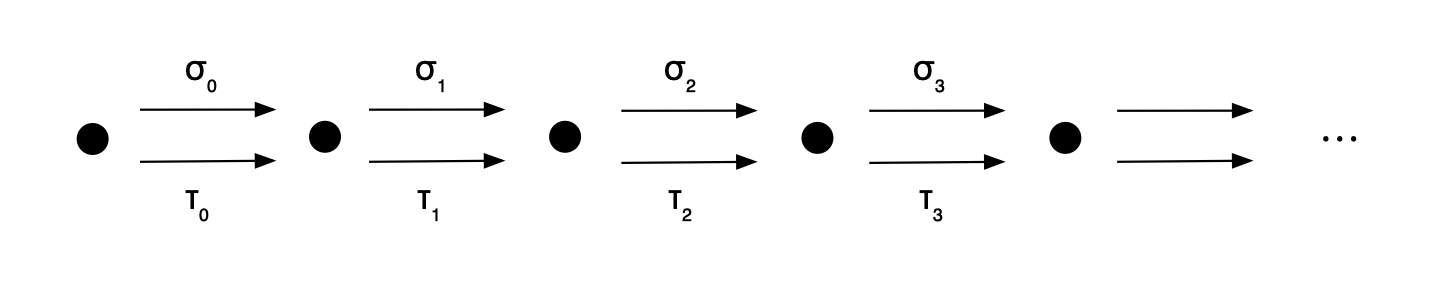
\includegraphics[scale=0.5]{globecat.png}
\end{center}

\href{https://ncatlab.org/nlab/show/globular+set}{Globular sets} are functors from the opposite category of the globe category 𝔾 into the category of sets, and maps of globular sets are natural transformations between them.\\

In this chapter we prove the following (which we have called Whitehead Theorem (c)): ∀(E:D(∞-Grpd₀)),∀(B:D(∞-Grpd₀)),∀(f:E ⭢ B),∀(G:E ⭢ B),(∀(n:Nat),(πₙ F = πₙ G)) ⭢ F = G, where πₙ is notation for π n.\\

This can be shown using CW-replacement and induction on n. Fibrant replacement of an object X entails replacing an object in ∞-Grpd₀ with a CW-object (an object made by successively glueing in higher and higher simplices along their boundaries obtaining a sequence Xₙ). Given an equality π${}_{n+1}(f) = $π${}_{n+1}(g)$ and a homotopy equivalence hₙ : Δ¹ × Xₙ ⭢ Y between $f|_{X_n}, g|_{X_n}$ : Xₙ ⭢ Y, we construct an extension of the homotopy equivalence Δ¹ × $X_{n+1}$ ⭢ Y.\\

\iffalse
Can the attaching map be 
\fi

{\bf Spheres and balls} Next we turn to defining spheres and balls:

{
\footnotesize
\begin{center}
\begin{tabular}{||l || l || l ||} 
 \hline
  & \multicolumn{2}{||c||}{\texttt{Spheres and Balls}} \\
 \hline
 Name of the $\texttt{X}$ value & \texttt{∂X ≅ Sⁿ} & \texttt{X ≅ Dⁿ} \\
 \hline
 \hline
 p-norm unit ball for p = 1 & ∂B(1,1) & B(1,1) \\
 \hline
 p-norm unit ball for 1 < p < 2 & ∂B(p,1) & B(p,1) \\
 \hline
 p-norm unit ball for p = 2 & ∂B(2,1) & B(2,1) \\
 \hline
 p-norm unit ball for 2 < p < ∞ & ∂B(p,1) & B(p,1) \\
 \hline
 p-norm unit ball for p = ∞ & ∂B(∞,1) & B(∞,1) \\
 \hline
 The n-simplex & ∂Δⁿ & Δⁿ \\
 \hline
 \hline
\end{tabular}
\end{center}
}

\begin{definition}
...
\end{definition}

\iffalse
\begin{definition}
Define a function d${}^{(n_1,...,n_k)} : $ D${}^{n_1}$ × $\cdots$ × D${}^{n_k}$ ⭢ D${}^{n_1 + \cdots + n_k}$ sending $(x_1,...,x_k)$...
\end{definition}
\fi

\begin{theorem}
i¹ : S⁰ ⭢ D¹ 
\end{theorem}

\begin{theorem}
Dⁿ × D¹ ⭢ Dⁿ⁺¹
\end{theorem}

\begin{definition}
Dⁿ ⭢ Dᵐ
\end{definition}


\begin{theorem}
Fix n : ℕ and let ∂ⁿ : Sⁿ ⭢ Dⁿ⁺¹ be the inclusion. The pushout of the following diagram is isomorphic to Sⁿ⁺¹:
\begin{center}
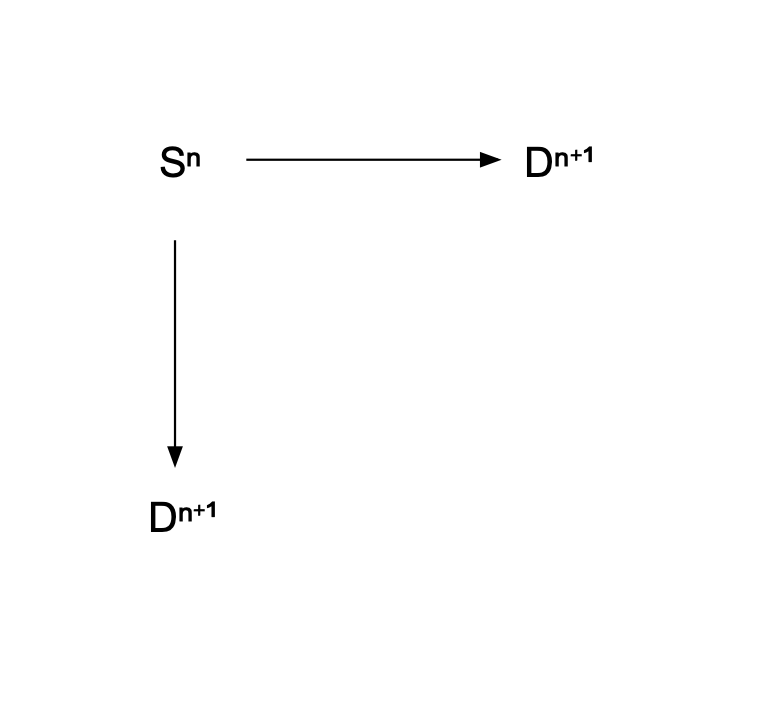
\includegraphics[scale=0.5]{pushout.png}
\end{center}
\end{theorem}

\begin{proof}

\end{proof}


\begin{theorem}
Define a function ||-||${}_{2}$ : Dⁿ ⭢ I sending (x₁,...,xₙ) to $\sqrt{\sum_{i = 1}^n x_i^2}$, and write ||-||${}_{2}$
\end{theorem}

\begin{proof}
...
\end{proof}

\section{HEP for based connected ∞-groupoids}

In this section we prove the homotopy extension property for based connected ∞-groupoids, which we here model as CW-complexes.\\


{\bf Jar filling} Next we turn to defining `jar shapes' $\texttt{Jⁿ}$, which include into $\texttt{Dⁿ × I}$ $\texttt{iₙ : Jⁿ ⭢ Dⁿ × I}$, after which we `fill' them (i.e. demonstrate that any continuous map f : Jⁿ ⭢ X extends to a continuous map g : Dⁿ × I ⭢ X).\\

The first and most common approach involves `shining a light ray down from above the jar', i.e. projection. We obtain a formula for .\\

The second way to fill the jar



\iffalse
In what follows, it is possible to use cell complexes instead of CW-complexes. This reflects how the argument makes no use of the stronger condition associated to the CW-complexes that cells be attached in order of nondecreasing dimension.
\fi

{\bf Change of Base} Jar filling leaves the question

\begin{definition}
Let X₋₁ be a connected CW-complex and let n : Nat be a natural number. The transport function $\texttt{trans\ n\ X₋₁ : (f : [I,X₋₁])  → πₙ (f 0) ⭢ πₙ (f 1)}$ is 
\end{definition}

\begin{theorem}
Let X₋₁ be a connected CW-complex and let f : I ⭢ X₋₁ be a path, so that $\texttt{(trans\ n X₋₁ f⁻¹) • (trans\ n X₋₁ f)}$ has type $\texttt{πₙ (f 0) ⭢ πₙ (f 0)}$. Then
\begin{center}
$\texttt{(trans\ n X₋₁ f⁻¹) • (trans\ n X₋₁ f) = 1\_(πₙ (f 0))}$
\end{center}
\end{theorem}

\begin{proof}
...
\end{proof}

The proof in the above can be depicted like so, as a `painting with two concentric frames':

\begin{center}
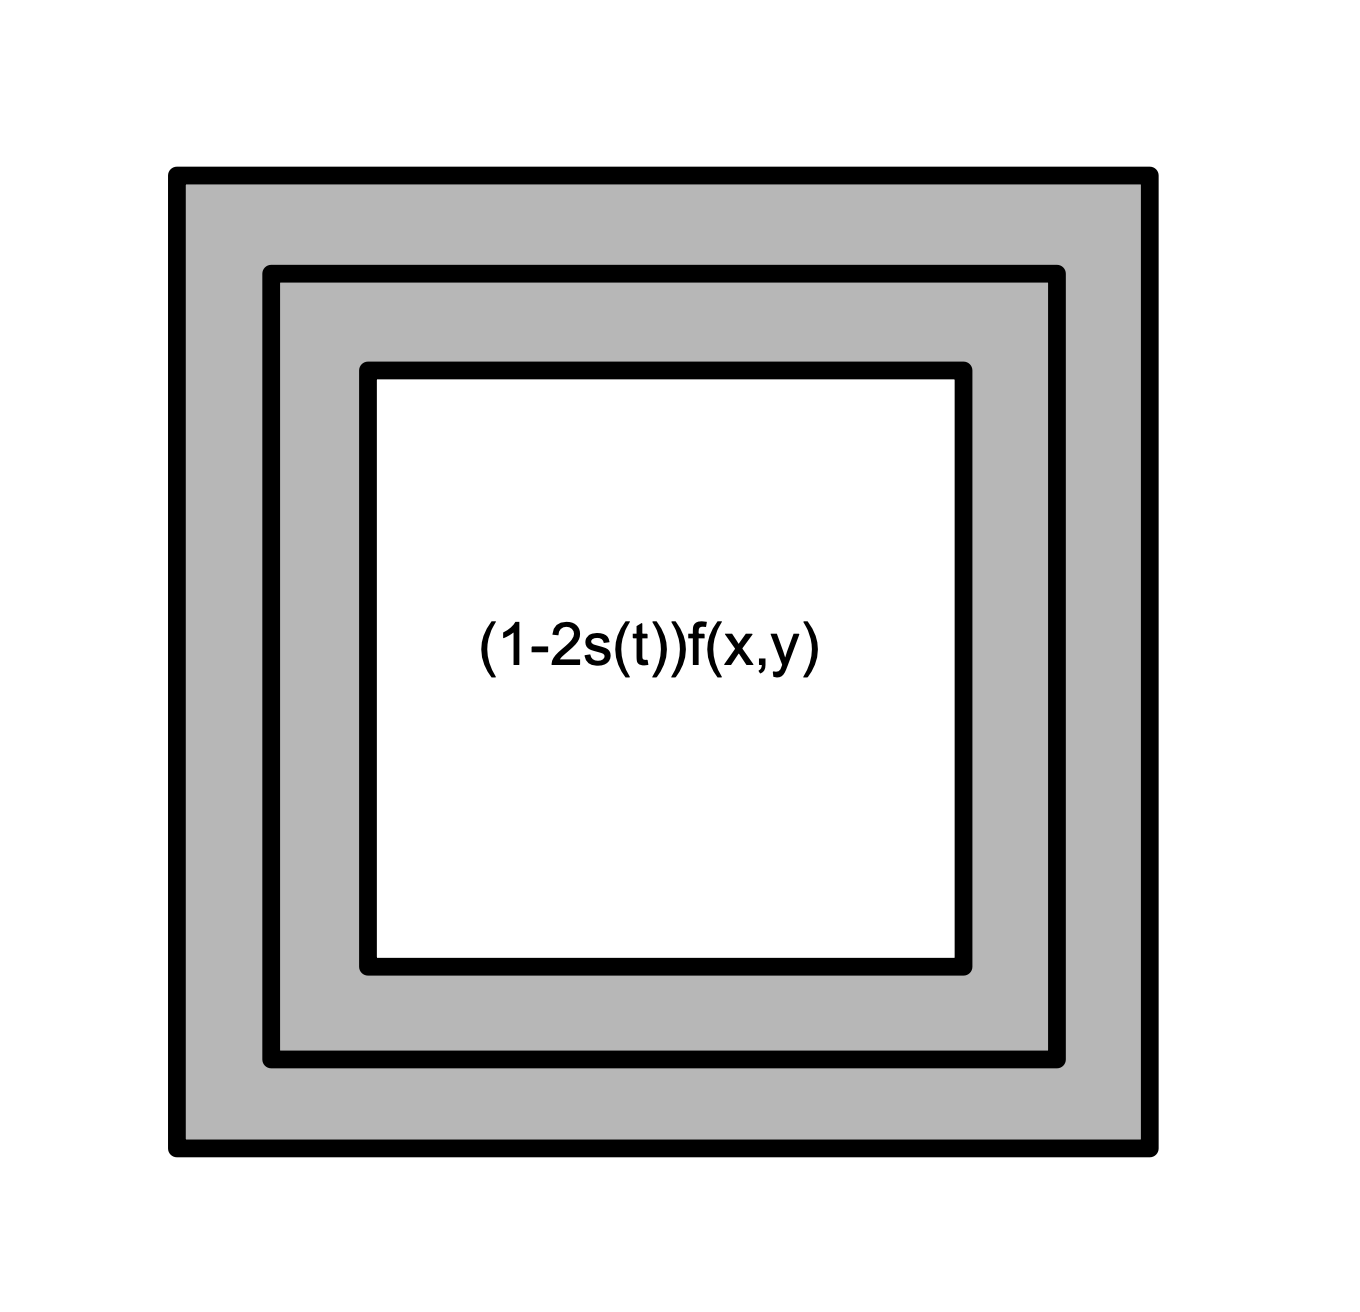
\includegraphics[scale=0.5]{windowframe.png}
\end{center}

that the based CW-complexes (X₋₁,x) and (X₋₁,y) are 

\begin{theorem}

\end{theorem}

\begin{proof}
...
\end{proof}

\begin{center}
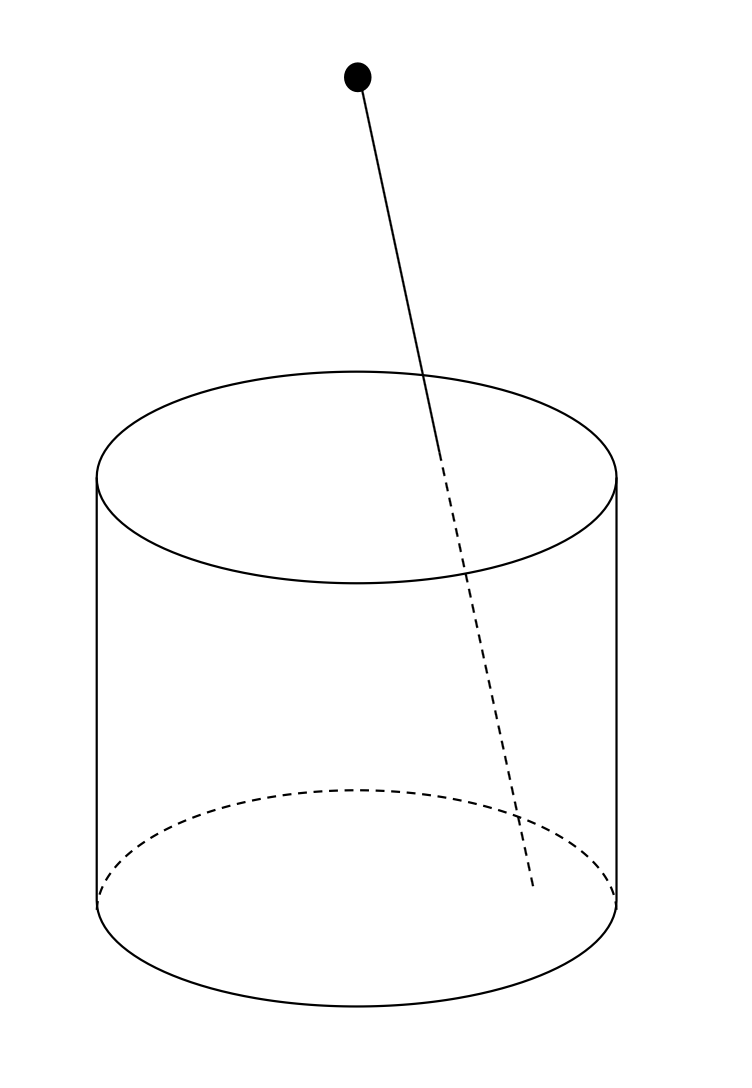
\includegraphics[width=3.5cm,height=5cm]{proj.png}
\end{center}

 



\section{REP for based connected ∞-groupoids}

In this section we use the notion of globular sets to replace a topological space with a CW-complex. Together with HEP (homotopy extension), this will complete the proof of the Whitehead theorem.


\section{The Whitehead theorem}

Here we show the Whitehead theorem.

\iffalse
https://leanprover-community.github.io/mathlib4_docs/Mathlib/Topology/Homotopy/HomotopyGroup.html
\fi

\iffalse
In proving the Whitehead theorem formally, \textit{we make use of a line} as well as, in essence, the structure of a \textit{groupoid} $\texttt{G}_{\texttt{X}}$ where $\texttt{Hom}{}_{\texttt{G}}\texttt{(x,x)}$ is taken to be πₙ(X,x). This interesting feature of the proof relates to the other two Whitehead theorems featuring categories π⃗ₙ and groupoids π⃡ₙ.\\
\fi


\chapter{Chapter 3: The Category of Pairs}

In this section I would like to 



\chapter{Chapter 4: Internal and Operadic Groups}

\iffalse
An operadic group is an algebra for the little lines operad, which has ??? entries

An operadic internal group in an ∞-category C is an algebra for the little lines internal operad, which has ??? entries.
\fi

\section{\texttt{InternalGroup}}

%LEAN: internal_group
\begin{center}
\begin{tcolorbox}[width=5in,colback={white},title={\begin{center}\texttt{Lean \thelcounter} \addtocounter{lcounter}{1}  \end{center}},colbacktitle=Blue,coltitle=black]
\begin{minted}[breaklines, escapeinside=||]{lean}

/-
structure internal_group ... where
  Obj := D(Γ).Obj
-- Dom := 
-- Cod
-- Idn
-- Fst
-- Snd
-- Cmp
-- Id₁
-- Id₂
-- Ass
-- Com
-/

\end{minted}
\end{tcolorbox}
\end{center}


\section{\texttt{InternalGroupAction G}}

Here we define internal group actions. These will be important when we talk about G-principal bundles (themselves defined as internal group actions in the derived category of an overcategory). 


\section{\texttt{OperadicGroup}}




\section{\texttt{OperadicGroupActions}}



\section{The \texttt{O} and \texttt{P} Functors}

The internal group principal stems from the simple observation that the loop space forms a component of an internal group.\\


\section{The \texttt{o} and \texttt{p} Functors}

The internal group actions principal stems from the simple observation that the homotopy fiber forms a component of an internal group action.\\



\part{∞-GROUPOIDS}

The Whitehead theorem is about the ways that spheres can get stuck in spaces (higher homotopy groups), and the last section established how these higher homotopy groups relate to maps in the homotopy category of based connected CW-complexes. There is the nuance that the base .\\


\chapter{Chapter 9: ∞\texttt{-Grpd}}


\section{Ω⃡}

Our choice of symbols refects our choice of three variations of the Whitehead theorem and three Puppe sequences. Ω⃡, the analogue of loop space, is the internal hom functor [I,-] : ∞-Grpd ⭢ ∞-Grpd. This is not hard to construct, with the main lemma being that the path space of a quasicategory has the quasicategory lifting conditon.\\

We will be interested in one formal model of D(∞-Cat) which consists of formal compositions f₁ • g₁ • f₂ • g₂ • ⋯ • fₙ • gₙ, where gₙ $: Dom(f{}_{n+1}) $⭢ ??? is a weak equivalence, and something similar for D(∞-Cat). However, it is still vital to have the replacement functor $\texttt{repl}$, which ensures the Whitehead theorem for particular ∞-categories which are constructed out of attaching maps.\\


\section{ω⃡}

Ω⃗ is to internal categories as ω⃡ is to internal G-actions. It is also called directed homotopy pullback. These functors will later be used to produce functors P⃡ : D(∞-Grpd) ⭢ InternalCategory D(∞-Grpd) and p⃡ : D(∞-Grpd⁄C) ⭢ InternalPresheaf (P⃡ G) D(∞-Grpd⁄G).\\


\section{π⃡ₙ}

The mentioned functors π⃡ₙ are designed with both Whitehead theorem (a) and Puppe sequence (a) in mind.\\




\chapter{Chapter 10: The Whitehead Theorem for ∞-Groupoids}


\section{Cubical Complexes}

...\\

\iffalse
In this chapter, we take on the objective of Whitehead theorem (a), out of which we will prove the other more concrete Whitehead theorems:\\

\begin{center} ∀(E:D(∞-Cat)),∀(B:D(∞-Cat)),∀(F:E ⭢ B),∀(G:E ⭢ B),(∀(n:Nat),(π⃗ₙ F = π⃗ₙ G)) ⭢ F = G
\end{center}

We can attempt to form a slightly different category, much like the above, called 𝓓(∞-Cat), at first, and in a formal way, so as to create a category whose object component 𝓓(∞-Cat).α matches the object component ∞-Cat.α while featuring the above theorem in a formal way. However, with this as our model of D(∞-Cat), we may then also be interested in the establishment of a model in which the Whitehead theorem is demonstrated, with the main idea being to prove two complementary concepts:

\begin{enumerate}
\item (REP) Establish ``weak equivalent fibrant replacement" R : ∞-Cat.α ⭢ ∞-Cat.α (.α gives the object component in Mathlib's category theory library), analogous to CW-complex replacement in Whitehead's original paper. It's especially nice if R forms the object component of a functor F : ∞-Cat ⭢ ∞-Cat. D(F) : D(∞-Cat) ⭢ D(∞-Cat) should be a categorical equivalence, and that is what we will do.
\item (HEP) For the object R X, demonstrate that any F,G : (R X) ⭢ Y such that ∀(n:Nat),(π⃗ₙ F = π⃗ₙ G), there is a directed homotopy equivalence between F and G. Note that ``directed homotopy equivalence" consists of a composible sequence of simple directed homotopies Hᵢ : Δ¹ × (R X) ⭢ Y, 1 ≤ i ≤ n, with even Hᵢ running reverse to the odd Hᵢ.
\end{enumerate} 

Both of these will use induction on Lean's $\texttt{Nat}$. The first of these could be called a REP (for REplacement Property, but this isn't usual terminology), and the second typically uses induction and a HEP (Homotopy Extension Property). Our REPa will consist of objects made out of particular kinds of pushouts called attaching maps, and can be made functorial. Proving the HEPa can be done by well-order induction on the attaching maps present in our choice of R, thereby reducing to the case of extending a homotopy along a single attachment.\\

Our HEPa (directed box filling) is similar to the HEP shown in Whitehead's original paper, and to the approach detailed in Hatcher's textbook, though no doubt modified to suit our two goals:

\begin{enumerate}[(I)]
\item The analogue of the Puppe sequence on the front cover needs to hold.
\item The first Whitehead theorem on the front cover needs to hold.
\end{enumerate}

These two considerations determine our choice of π⃗ₙ, Ω⃗, and ω⃗. We take Ω⃗ to be (simply) the internal hom functor [Δ¹,-] (which requires showing that Ω⃗X has the inner-horn filling condition). ω⃗ is then defined as a certain pullback of Ω⃗, and π⃗ₙ is designed to produce a Puppe sequence with a meaningful notion of exactness by which we can demonstrate the goal of recognition theorems (i) and (ii). Specifically, it makes sense to use cubes in our definition of π⃗ₙ because of how they are representing objects of Ω⃗ⁿ. Meanwhile, it is also clear that the quotient producing π⃗ₙ is subtle in exactly how it requires fixing the endpoints of a sequence of alternating directed homotopies. We will define π⃗ₙ's by identifying those objects x, y: Ω⃗ⁿ X which are homotopic by a homotopy which restricts to a constant along the face maps fᵢ : Ω⃗${}^{n-1}$ X ⭢ Ω⃗${}^{n-1}$ X (which correspond to pairs (n,b), where b : Bool).\\

Imagine for a moment the picture of a square shaped cusion; we might make such a cusion by first soeing together 6 squares of cloth and filling it with material, then "soeing the walls down to a square". Here we go with this:

\begin{enumerate}
\item Define a n-cubical cusion using the boundary of an n-1 cube times Δ¹, i.e. the quotient of (Δ¹)${}^{n-1}$ × Δ¹ by an equivalence relation, but we have to start our model somewhere), or perhaps more easily the pushout of f : Δ¹ × (∂((Δ¹)ⁿ)) ⭢ (Δ¹)${}^{n+1}$ by the projection map Δ¹ × (∂((Δ¹)ⁿ)) ⭢ ∂((Δ¹)ⁿ)
\item Define a simplicial cusion using the boundary of an n-1 simplex times Δ¹, i.e. the quotient of (Δ¹) by an equivalence relation, or perhaps more easily the pushout of f : Δ¹ × (∂(Δⁿ)) ⭢ (Δ¹) × Δⁿ by the projection map Δ¹ × (∂((Δ¹)ⁿ)) ⭢ ∂(Δⁿ)
\end{enumerate}

The boundary of a cusion is a pouch, isomorphic to a pushout of two cubes glued together at their boundaries:

\begin{enumerate}
\item Define a n-cubical pouch as the pushout of two boundary maps ∂((Δ¹)ⁿ) ⭢ (Δ¹)ⁿ
\item Define a simplicial pouch as the pushout of two boundary maps ∂(Δⁿ) ⭢ Δⁿ
\end{enumerate}

Notice that paths in Ω⃗ⁿX produce paths in Ω⃗${}^{n-1}$X in as many ways as there are face maps (Δ¹)${}^{n-1}$ ⭢ Δ¹${}^{n}$, these could be called restrictions and are no doubt related to the pouches and cusions we just defined. The cartesian closed structure on simplicial sets with the lifting condition clarifies the relationship between the two available definitions of π⃗ₙ:

\begin{enumerate}
\item Homotopies of maps from a cube which are constant on the boundary
\item Paths of maps in Ω⃗${}^{n-1}$X which produce constant maps under the mentioned restritions.
\item Maps from a pouch mod an equivalence relation (really we phrase this as a pushout!), namely the equivalence relation in which any two maps from a pouch that extend to maps from a cusion are identified.
\end{enumerate}

After we construct π⃗ₙ in the first section, we will be in a place to demonstrate that the natural transformation $\texttt{weak\_equivalence : repl ⭢ (𝟙 }$∞$\texttt{-Cat)}$ consists of weak equivalences (a fact which we call REP, which is short for REplacement Principal). This is covered in the section titled REP, which also constructs $\texttt{repl}$ and $\texttt{weak\_requivalence}$.\\

In sum, the goal of the present chapter is to use similar insights to the proof of the Whitehead theorem featured Hatcher's textbook to prove Wa and Pa for the model of quasicategories, using Mathlib's predefined horns and simplices in its simplicial sets section. The main difference is that our work must take care to respect the directed nature of quasicategories.\\
\fi

\iffalse
In the future, we intend to add important aspects of the bigger picture besides those which directly establish REP and HEP in the sections below. These are important considerations in ensuring usability. Three different model structures on ∞-Cat ensue from the six definitions below, which are contained in Lurie's ``Higher Topos Theory" on page 53, and which are due to Joyal:

\begin{definition} A morphism $\texttt{f : X ⭢ S}$ of simplicial sets is
\begin{enumerate}
\item A left fibration if f has the right lifting property with respect to all
horn inclusions Λni ⊆ ∆n, 0 ≤ i < n.
\item A right fibration if f has the right lifting property with respect to all
horn inclusions Λni ⊆ ∆n, 0 < i ≤ n.
\item An inner fibration if f has the right lifting property with respect to all
horn inclusions Λni ⊆ ∆n, 0 < i < n.
\end{enumerate}
A morphism of simplicial sets $\texttt{i : A ⭢ B}$ is
\begin{enumerate}
\item left anodyne if $\texttt{i}$ has the left lifting property with respect to all left fibrations.
\item right anodyne if $\texttt{i}$ has the left lifting property with respect to all right fibrations.
\item inner anodyne if $\texttt{i}$ has the left lifting property with respect to all inner fibrations.
\end{enumerate}
\end{definition}
\fi

\begin{enumerate}
\item Defining $\texttt{repl}$
\item 
\end{enumerate}


\section{REP}

We have divided the work of proving Whitehead theorem (a) into two steps: REP and HEP. In this section, we construct a functor $\texttt{repl : }$∞$\texttt{-Cat ⭢ }$∞$\texttt{-Cat}$ along with a natural transformation $\texttt{weak\_equivalence : repl ⭢ (𝟙 }$∞$\texttt{-Cat)}$. To construct $\texttt{repl}$ 



\section{HEP}

Consider the context of , supposing that we have constructed a homotopy ... This gives a picture that is a bit like ``filling up a jar``: a homotopy h : of f, g : ∂Δ² ⭢ Y, along with the value of g on Δ², produces a ``jar" shape in Y, which can be ``filled up" to produce a homotopy h : Δ¹ × Δ² ⭢ Y. This is easier for simplicial-based approaches than for point-set topological approaches, the latter of which needs extra steps that deform a map into a cellular map.\\

This construction, in the case of point set topology, often involves first deforming maps so as to be cellular; however our analogue of CW complexes allows us to skip this step.\\

This construction (HEP for quasicategories) may even be equivalent to the quasicategory lifting condition if we are lucky. It is also the main technical device allowing for our concrete choice of model (quasicategories).\\

In this section, we demonstrate this extension property and use it to conclude the Whitehead theorem for ∞-categories stated above.\\

\begin{center}
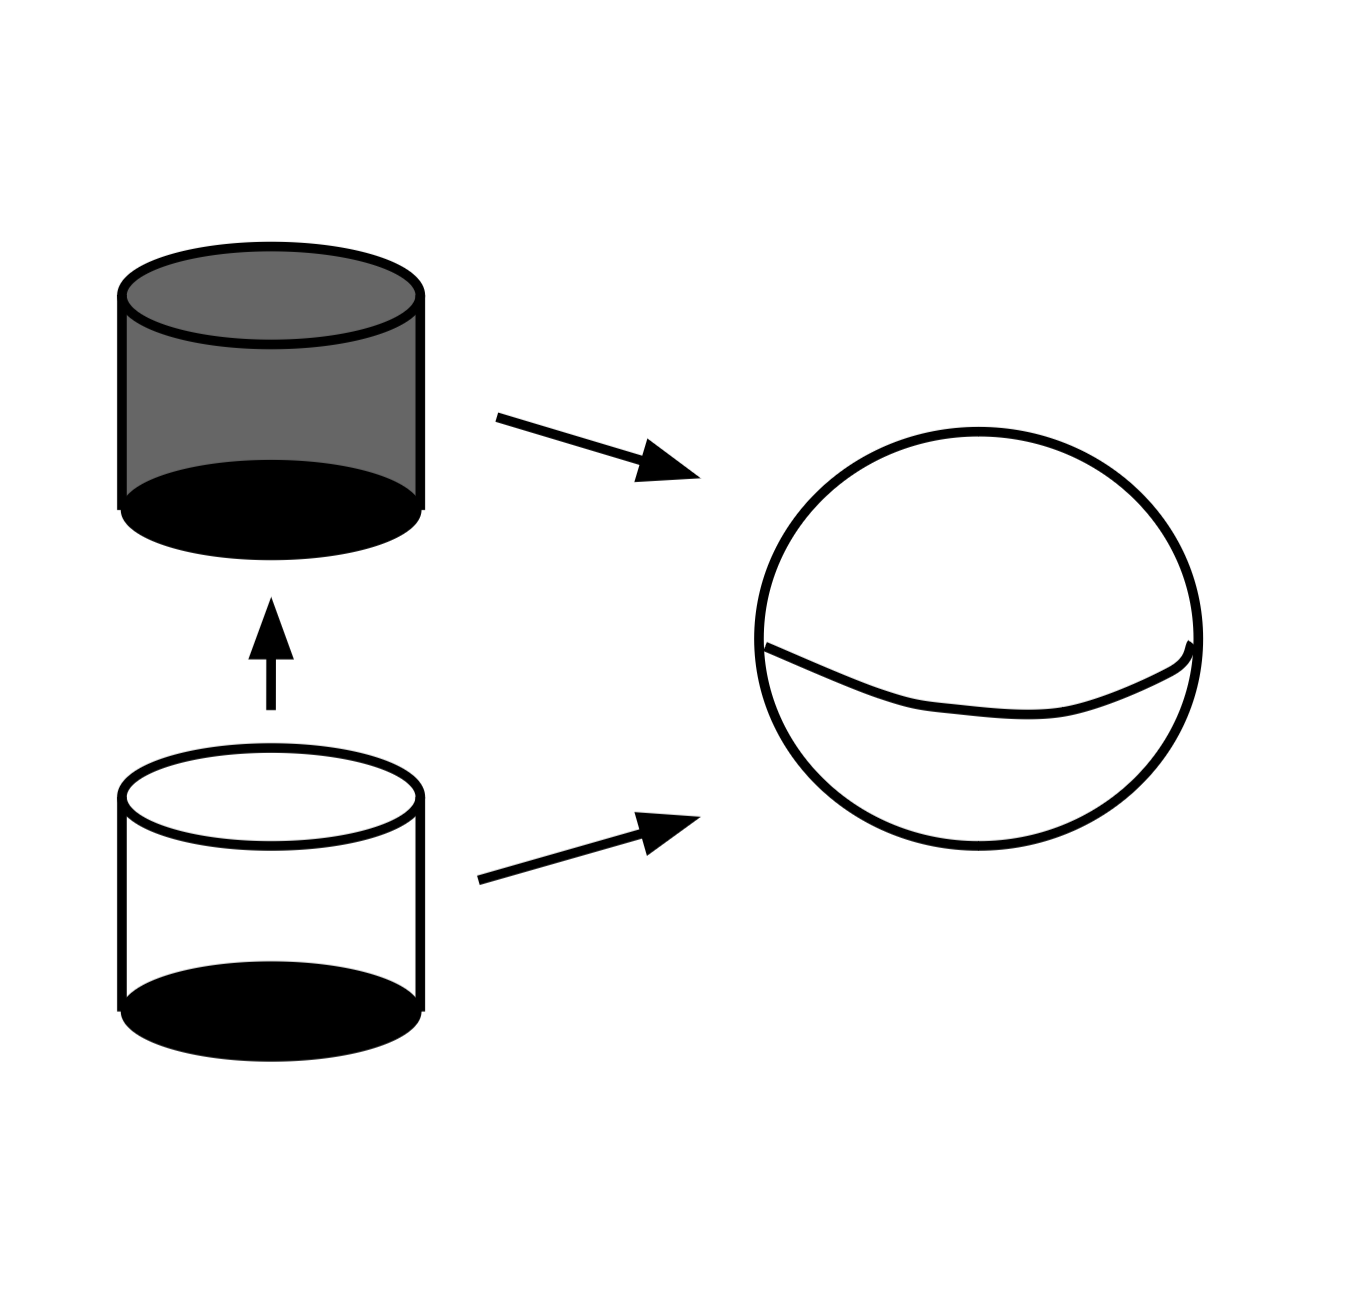
\includegraphics[width=0.5\textwidth]{HEP.png}
\end{center}

{\bf Prism Filling (PF)} Let Y be a quasicategory, and let f, g : ∂Δⁿ ⭢ Y. A homotopy h : ∂Δⁿ × Δ¹ ⭢ Y between f, g : ∂Δⁿ ⭢ Y extends to a map H : Δⁿ × Δ¹ ⭢ Y; this follows from the condition that Y be a quasicategory. H(-,1) and g match on ∂Δⁿ, producing a map f : X ⭢ Y, where X consists of two copies of Δⁿ glued together at the boundary. Consider a space X' formed as a quotient of Δⁿ × Δ¹ by ∂Δⁿ × Δ¹. There is a map φ : X ⭢ X'. An induction hypothesis on f and g involving πₙ ensures that the aparent map X ⭢ Y lifts along φ, producing a map from Δⁿ × Δ¹ which is constant on ∂Δⁿ × Δ¹. Stacking this on top of H can be done using an isomorphism between Δ¹ and Δ¹ glued with itself along different endpoints. Altogether this produces a homotopy between f and g.\\

Directed prism filling may combine fruitfully with the yoneda lemma and/or the fact that simplicial sets are determined by the sets [Δⁿ,X] along with combinatorial information (face and degeneracy maps).

{\bf Decomposing Δⁿ × Δ¹ into a colimit involving n+1 Δ${}^{n+1}$'s} ...

\begin{center}
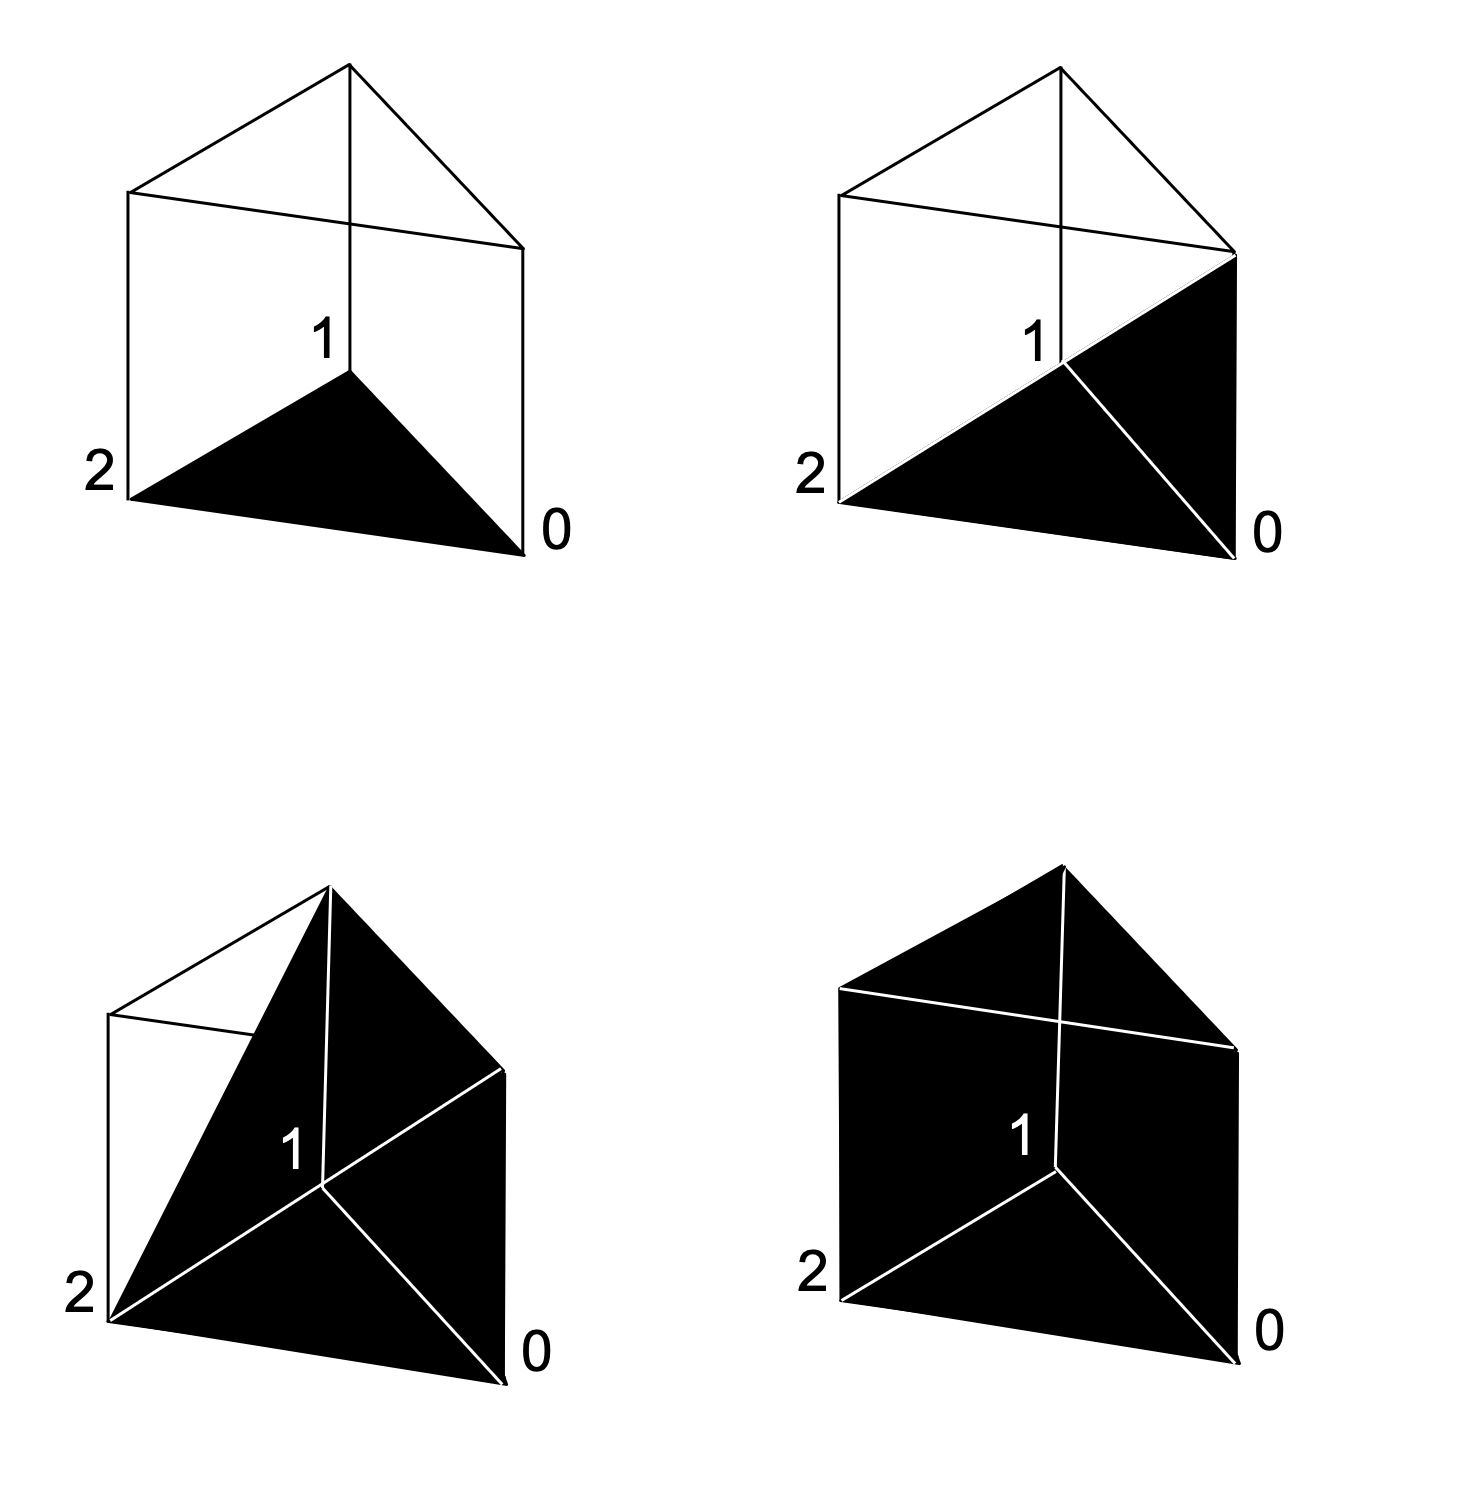
\includegraphics[width=300pt]{prismfilling.png}
\end{center}

In the above, it may be easier if we make use of sub-simplicial sets and prove the theorem using that colimit applied to a natural isomorphism of diagrams products an isomorphism.\\

The decomposition 

A definition of π⃗ₙ which is consistent with our goals of Wa and Pa is one as a certain pushout involving (Ω⃗ⁿ X)-- one which amounts to taking an equivalence relation by paths in Ω⃗ⁿ X which restrict to constant paths along the face maps fᵢ : Ω⃗${}^{n-1}$ X ⭢ Ω⃗ⁿ X. Here, Ω⃗ is easy to define in the model of quasi-categories, and it amounts . Besides fullfilling our goal of the first Whitehead theorem and puppe sequence, this definition of π⃗ₙ strikes me as elegant because it uses all of the ways for Ω⃗ⁿ X to map into Ω⃗${}^{n+1}$ X.\\

The next symbols in the project's ``periodic table" that we construct, after Ω⃗ and π⃗ₙ, will be B⃗ and E⃗, which we feature in the chapter on Puppe sequence (a).\\

A useful thing for us to construct first is the boundary of a product of Δ¹'s and the boundary of a directed simplex. We might even like to expand on this later, but for now just consider for a moment how each might be made out of a glueing construction involving face maps.\\

Even though the π⃗ₙ's can be defined using Ω⃗ⁿ X and various face maps f$\_(n,b)$ : Ω⃗${}^{n-1}$ X ⭢ Ω⃗${}^{n}$ X for $b : \{ 0, 1 \}$, it may be nice to have this as a result, with the definition one featuring two cubes glued together along their boundary.\\

This means that we want directed box filling in addition to directed prism filling (but which also uses directed prism filling in its proof).

{\bf Box Filling (BF)} Let Y be a quasicategory, and let f, g : ∂Δⁿ ⭢ Y. A homotopy h : ∂Δⁿ × Δ¹ ⭢ Y between f, g : ∂Δⁿ ⭢ Y extends to a map H : Δⁿ × Δ¹ ⭢ Y; this follows from the condition that Y be a quasicategory. H(-,1) and g match on ∂Δⁿ, producing a map f : X ⭢ Y, where X consists of two copies of Δⁿ glued together at the boundary. Consider a space X' formed as a quotient of Δⁿ × Δ¹ by ∂Δⁿ × Δ¹. There is a map φ : X ⭢ X'. An induction hypothesis on f and g involving πₙ ensures that the aparent map X ⭢ Y lifts along φ, producing a map from Δⁿ × Δ¹ which is constant on ∂Δⁿ × Δ¹. Stacking this on top of H can be done using an isomorphism between Δ¹ and Δ¹ glued with itself along different endpoints. Altogether this produces a homotopy between f and g.\\

This goes hand-in-hand with a definition of π⃗ₙ which suits (I) and (II) in the introduction to chapter (3). If we make sure to prove lemmas... 

The box filling and prism filling HEPs can be extended to the case of attaching all cells of a particular fixed dimension and as indexed by simplicial set arising from a set (or Lean 4 $\texttt{Type}$). That is, we might like to extend × $()$ (or possibly somehow a $\texttt{Set}$ as well), and that we may find an interest in the following two definitions of π⃗ₙ, which are designed to fullfill both (I) and (II) in the chapter's introduction.\\

Breaking down BF further can be done conveniently using sub-simplicial sets, just like we used in the proof of prism filling. 

\begin{center}
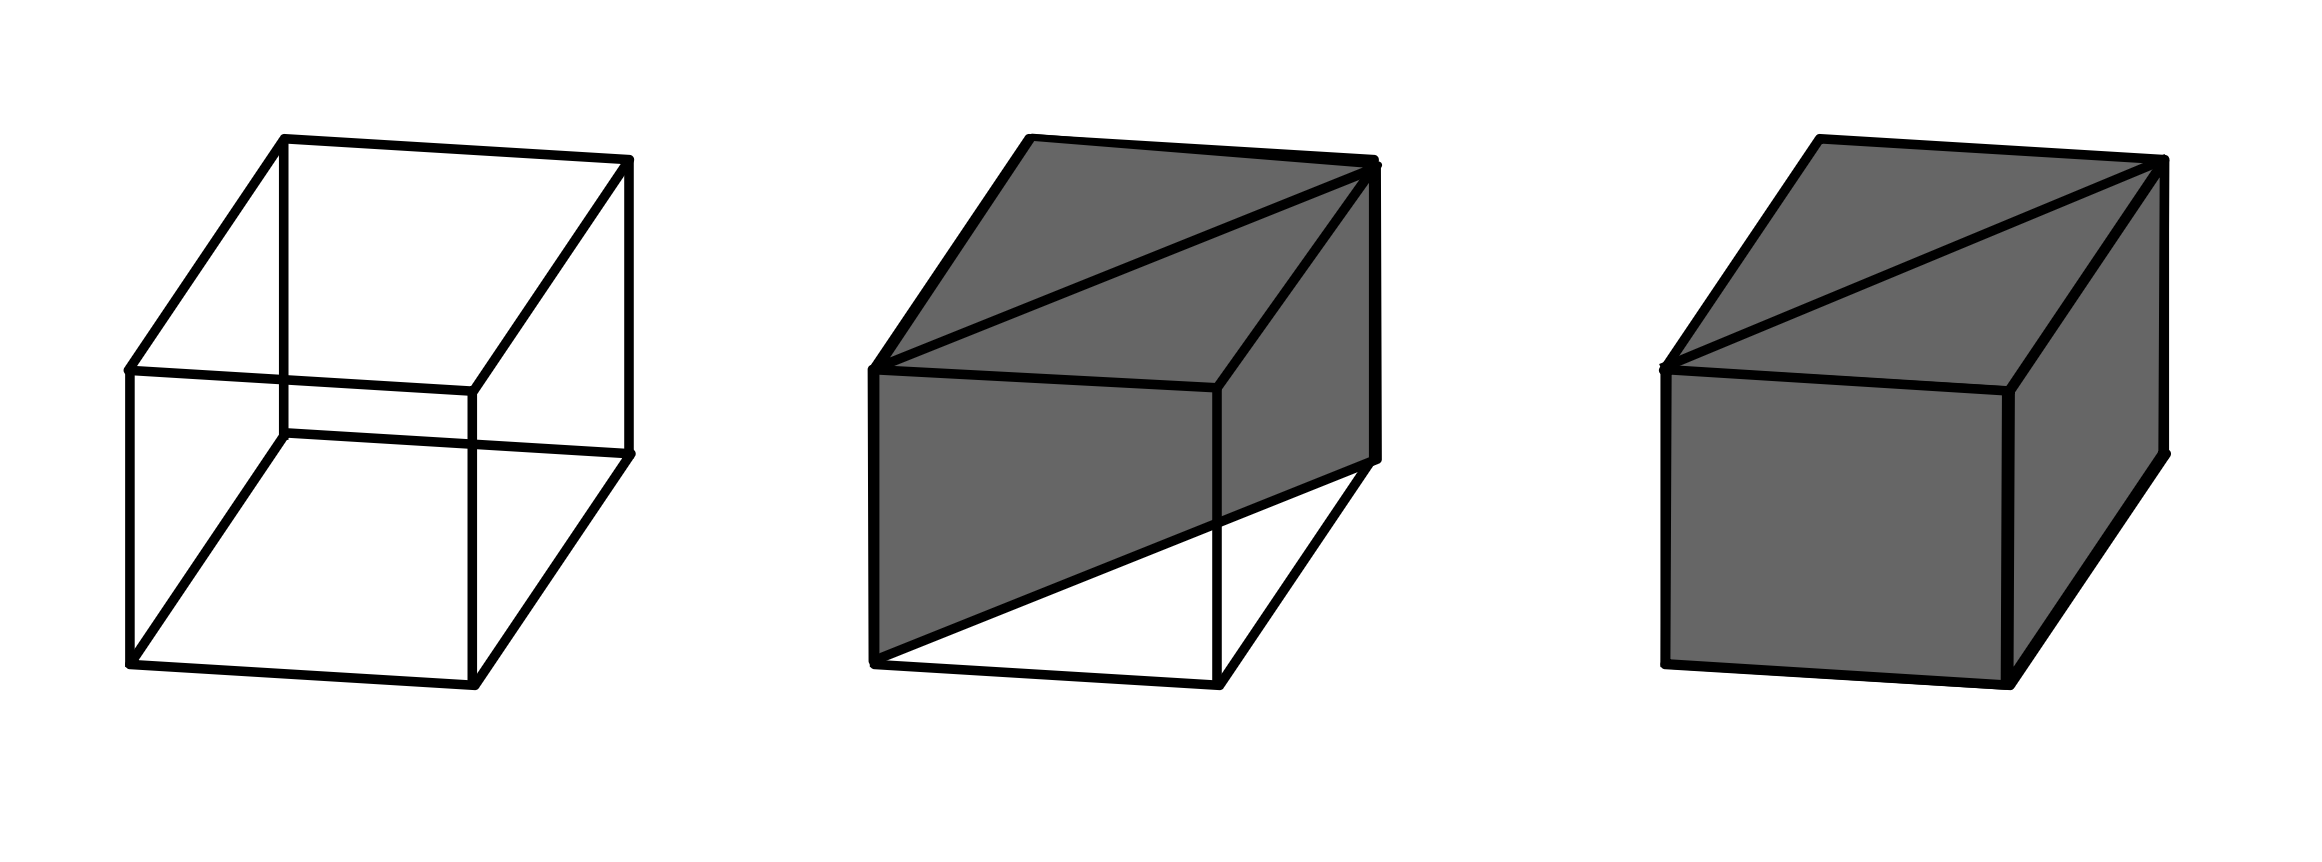
\includegraphics[width=300pt]{boxfilling.png}
\end{center}


{\bf Decomposing (Δ¹)ⁿ into a colimit involving n! Δⁿ's} Consider the face maps fᵢ : Δⁿ ⭢ Δ${}^{n+1}$


The decomposition 
The box filling lemma allows us to prove HEP:


The HEP in the last 

..H(-,1) and g match on ∂Δⁿ, producing a map f : X ⭢ Y, where X consists of two copies of Δⁿ glued together at the boundary. Consider a space X' formed as a quotient of Δⁿ × Δ¹ by ∂Δⁿ × Δ¹. There is a map φ : X ⭢ X'. An induction hypothesis on f and g involving πₙ ensures that the aparent map X ⭢ Y lifts along φ, producing a map from Δⁿ × Δ¹ which is constant on ∂Δⁿ × Δ¹. Stacking this on top of H can be done using an isomorphism between Δ¹ and Δ¹ glued with itself along different endpoints. Altogether this produces a homotopy between f and g.\\

Imagine 


\chapter{Chapter 11: The Category of Pairs of ∞-Groupoids}




\chapter{Chapter 12: Internal and Operadic Groupoids and their Actions}

\iffalse
An operadic groupoid is an algebra for the little lines operoid with ??? entries

An operadic internal groupoid in C is an algebra in C for the little lines internal operoid with ??? entries
\fi

In this chapter, we discuss internal categories and internal presheaves in a pullback system. We may keep in mind that internal categories and internal presheaves can be formed in any category with pullbacks, even though we focus on the case of pullback systems because of our interest in Whitehead theorem (a).\\

After defining the category of internal categories D(Γ), we proceed to observe how, for C , D : D(Γ), F : C ⭢ D, (ω⃗ F).obj F forms an internal categry. Further, in considering internal (P⃗\_(Γ) F)-presheaves for  C , D : D(Γ), F : C ⭢ D, we proceed to make observations about (ω⃗ F).obj G.\\

{
\footnotesize
\begin{center}
\begin{tabular}{||l || l ||} 
 \hline
 $\texttt{Section}$  &\ $\texttt{Description}$ \\
 \hline \hline
 $\texttt{InternalGroupoid : Cat}$   &\ Internal categories \\ 
 \hline
 $\texttt{InternalGroupoidAction G : Cat}$ &\ Internal C-presheaves \\ 
 \hline
 The internal category principal &\ \texttt{f ×\_(B) f} forms an internal category\\
 \hline
 The internal presheaf principal &\ \texttt{f ×\_(B) f} forms an internal presheaf\\
 \hline
 P⃗ C : InternalCategory D(∞-Cat) &\ Ω⃗ C forms a component of an internal category \\
 \hline
 p⃗ (𝟙 C) D : InternalPresheaf D(∞-Cat⁄C) (P⃗ C) &\ ω⃗ (𝟙 C) D forms a component of an internal C-presheaf \\
 \hline
\end{tabular}
\end{center}
}

\section{\texttt{Internal Groupoids}}

In this chapter I define an \href{https://ncatlab.org/nlab/show/internal+category}{internal category}. Internal categories are most commonly defined on categories with enough pullbacks, but here I may also like to keep in mind that it is valuable to be able to iterate $\texttt{InternalGroupoid}$ in the way of composition.\\

%LEAN: definition of an internal groupoid in a pullback system
\begin{center}
\begin{tcolorbox}[width=5in,colback={white},title={\begin{center}\texttt{Lean \thelcounter} \addtocounter{lcounter}{1}  \end{center}},colbacktitle=Blue,coltitle=black]
\begin{minted}[breaklines, escapeinside=||]{lean}

-- definition of an internal category in a pullback system
/-
structure internal_groupoid (Γ : Cat) where
  Obj : .Obj
  Mor : .Obj
  Dom : .Hom Mor Obj
  Cod : .Hom Mor Obj
  Idn : .Hom Obj Mor
  Fst : .Cmp Obj Mor Obj Idn Dom  = 𝟙_(Γ.Obj) Obj
  Snd : .Cmp Obj Mor Obj Idn Cod = 𝟙_(Γ.Obj) Obj
--  Cmp : D(Γ).Γ.PulObj ...
-- Id₁ : D(Γ).
-- Id₂ : D(Γ).
-- Ass : D(Γ).
-/

\end{minted}
\end{tcolorbox}
\end{center}

The internal functor structure combines with the internal category structure to give a category of internal categories in a pullback system.\\

%LEAN: definition of an internal functor in a pullback system
\begin{center}
\begin{tcolorbox}[width=5in,colback={white},title={\begin{center}\texttt{Lean \thelcounter} \addtocounter{lcounter}{1}  \end{center}},colbacktitle=Blue,coltitle=black]
\begin{minted}[breaklines, escapeinside=||]{lean}

-- definition of an internal functor in a pullback system
structure internal_functor (Γ : pullback_system) (C : internal_category Γ) (D : internal_category Γ) where
  Obj : D(Γ).Hom C.Obj D.Obj
-- Mor : D(Γ).
-- Fst : D(Γ).
-- Snd : D(Γ).
-- Idn : D(Γ).
-- Cmp : D(Γ).

\end{minted}
\end{tcolorbox}
\end{center}


%LEAN: definition of the identity internal functor in a pullback system
\begin{center}
\begin{tcolorbox}[width=5in,colback={white},title={\begin{center}\texttt{Lean \thelcounter} \addtocounter{lcounter}{1}  \end{center}},colbacktitle=Blue,coltitle=black]
\begin{minted}[breaklines, escapeinside=||]{lean}

-- definition of the identity internal functor in a pullback system
def InternalCategoryIdn (Γ : pullback_system) (C : internal_category Γ) : (internal_functor Γ C C) := sorry

\end{minted}
\end{tcolorbox}
\end{center}

%LEAN: definition of the composition of internal functors in a pullback system
\begin{center}
\begin{tcolorbox}[width=5in,colback={white},title={\begin{center}\texttt{Lean \thelcounter} \addtocounter{lcounter}{1}  \end{center}},colbacktitle=Blue,coltitle=black]
\begin{minted}[breaklines, escapeinside=||]{lean}

-- definition of the composition of internal functors in a pullback system
def InternalCategoryCmp (Γ : pullback_system) (C : internal_category Γ) (D : internal_category Γ) (E : internal_category Γ) (F : internal_functor Γ C D) (G : internal_functor Γ D E) : (internal_functor Γ C E) := sorry

\end{minted}
\end{tcolorbox}
\end{center}

%LEAN: proving the first identity law for internal categories in a pullback system
\begin{center}
\begin{tcolorbox}[width=5in,colback={white},title={\begin{center}\texttt{Lean \thelcounter} \addtocounter{lcounter}{1}  \end{center}},colbacktitle=Blue,coltitle=black]
\begin{minted}[breaklines, escapeinside=||]{lean}

-- proving the the first identity law for internal categories in a pullback system
def InternalCategoryId₁ (Γ : pullback_system) (X : internal_category Γ) (Y : internal_category Γ) (f : internal_functor Γ X Y) : InternalCategoryCmp Γ X Y Y f (InternalCategoryIdn Γ Y) = f := sorry

\end{minted}
\end{tcolorbox}
\end{center}

%LEAN: proving the second identity law for internal categories  in a pullback system
\begin{center}
\begin{tcolorbox}[width=5in,colback={white},title={\begin{center}\texttt{Lean \thelcounter} \addtocounter{lcounter}{1}  \end{center}},colbacktitle=Blue,coltitle=black]
\begin{minted}[breaklines, escapeinside=||]{lean}

-- proving the second identity law for internal categories in a pullback system
def InternalCategoryId₂ (Γ : pullback_system) (X : internal_category Γ) (Y : internal_category Γ) (f : internal_functor Γ X Y) : (InternalCategoryCmp Γ X X Y (InternalCategoryIdn Γ X) f = f) := sorry

\end{minted}
\end{tcolorbox}
\end{center}

%LEAN: proving the associativity law for internal categories in a pullback system
\begin{center}
\begin{tcolorbox}[width=5in,colback={white},title={\begin{center}\texttt{Lean \thelcounter} \addtocounter{lcounter}{1}  \end{center}},colbacktitle=Blue,coltitle=black]
\begin{minted}[breaklines, escapeinside=||]{lean}

-- proving the associativity law for internal categories in a pullback system
def InternalCategoryAss (Γ : pullback_system) (W : internal_category Γ) (X : internal_category Γ) (Y : internal_category Γ) (Z  : internal_category Γ) (f : internal_functor Γ W X) (g : internal_functor Γ X Y) (h : internal_functor Γ Y Z) : InternalCategoryCmp Γ W X Z f (InternalCategoryCmp Γ X Y Z g h) = InternalCategoryCmp Γ W Y Z (InternalCategoryCmp Γ W X Y f g) h := sorry

\end{minted}
\end{tcolorbox}
\end{center}

%LEAN: defining the category of internal categories in a pullback system
\begin{center}
\begin{tcolorbox}[width=5in,colback={white},title={\begin{center}\texttt{Lean \thelcounter} \addtocounter{lcounter}{1}  \end{center}},colbacktitle=Blue,coltitle=black]
\begin{minted}[breaklines, escapeinside=||]{lean}

/-
def InternalCategory (Γ : pulback_system) : 𝐂𝐚𝐭.Obj := {Obj := internal_category Γ, Hom := internal_functor Γ, Idn := InternalCategoryIdn Γ, Cmp := InternalCategoryCmp Γ, Id₁ := InternalCategoryId₁ Γ, Id₂ := InternalCategoryId₂ Γ, Ass := InternalCategoryAss Γ}
-/

\end{minted}
\end{tcolorbox}
\end{center}

%LEAN: 
\begin{center}
\begin{tcolorbox}[width=5in,colback={white},title={\begin{center}\texttt{Lean \thelcounter} \addtocounter{lcounter}{1}  \end{center}},colbacktitle=Blue,coltitle=black]
\begin{minted}[breaklines, escapeinside=||]{lean}

-- notation : 2000 "Cat_(" Γ ")" => InternalCategory Γ

\end{minted}
\end{tcolorbox}
\end{center}

\section{\texttt{InternalGroupoidAction Γ C}}

The mentioned book $\textit{Galois Theories}$ by Janelidze and Borceux features a definition of internal presheaves for an internal groupoid in chapter 7 which makes a good reference for the present discussion.\\

%LEAN: internal C-presheaves
\begin{center}
\begin{tcolorbox}[width=5in,colback={white},title={\begin{center}\texttt{Lean \thelcounter} \addtocounter{lcounter}{1}  \end{center}},colbacktitle=Blue,coltitle=black]
\begin{minted}[breaklines, escapeinside=||]{lean}

-- internal C-presheaves
-- def internal_presheaf (C : (InternalCategory C).Obj) : Type := sorry

\end{minted}
\end{tcolorbox}
\end{center}

%LEAN: defining an internal functor between internal C-presheaves
\begin{center}
\begin{tcolorbox}[width=5in,colback={white},title={\begin{center}\texttt{Lean \thelcounter} \addtocounter{lcounter}{1}  \end{center}},colbacktitle=Blue,coltitle=black]
\begin{minted}[breaklines, escapeinside=||]{lean}

-- defining an internal functor between internal C-presheaves
/-
def Shfhom (C : (InternalCategory Γ).Obj) (F : internal_presheaf Γ C) (G : internal_presheaf Γ C) : Type := sorry
-/

\end{minted}
\end{tcolorbox}
\end{center}

%LEAN: defining the identity internal functor of an internal C-sheaf
\begin{center}
\begin{tcolorbox}[width=5in,colback={white},title={\begin{center}\texttt{Lean \thelcounter} \addtocounter{lcounter}{1}  \end{center}},colbacktitle=Blue,coltitle=black]
\begin{minted}[breaklines, escapeinside=||]{lean}

-- defining the identity internal functor of an internal C-sheaf
/-
def Shfidn (Γ : pullback_system) (C : (InternalCategory Γ).Obj) (F : internal_presheaf Γ C) : ShfHom Γ C F F := sorry
-/

\end{minted}
\end{tcolorbox}
\end{center}

%LEAN: defining the composition of internal functors
\begin{center}
\begin{tcolorbox}[width=5in,colback={white},title={\begin{center}\texttt{Lean \thelcounter} \addtocounter{lcounter}{1}  \end{center}},colbacktitle=Blue,coltitle=black]
\begin{minted}[breaklines, escapeinside=||]{lean}

-- defining the composition of internal functors
def Shfcmp (Γ : pullback_system) (C : (InternalCategory Γ).Obj) (F : internal_presheaf Γ C) (G : internal_presheaf Γ C) (H : internal_presheaf Γ C) (f : ShfHom Γ C F G)  (g : ShfHom Γ C G H) : ShfHom Γ C F H := sorry

\end{minted}
\end{tcolorbox}
\end{center}

%LEAN: proving the first identity law for internal functors
\begin{center}
\begin{tcolorbox}[width=5in,colback={white},title={\begin{center}\texttt{Lean \thelcounter} \addtocounter{lcounter}{1}  \end{center}},colbacktitle=Blue,coltitle=black]
\begin{minted}[breaklines, escapeinside=||]{lean}

-- proving the first identity law for internal functors
/-
def Shf... (Γ : pullback_system) (C : (InternalCategory Γ).Obj) (X : internal_presheaf Γ C) (Y : internal_presheaf Γ C) (f : ShfHom Γ C X Y) : ((ShfCmp Γ C X Y Y f (ShfIdn Γ C Y)) = f) := sorry
-/

\end{minted}
\end{tcolorbox}
\end{center}

%LEAN: proving the second identity law for internal functors
\begin{center}
\begin{tcolorbox}[width=5in,colback={white},title={\begin{center}\texttt{Lean \thelcounter} \addtocounter{lcounter}{1}  \end{center}},colbacktitle=Blue,coltitle=black]
\begin{minted}[breaklines, escapeinside=||]{lean}

-- proving the second identity law for internal functors
/-
def ShfId₂ (Γ : pullback_system) (C : (InternalCategory Γ).Obj) (X : internal_presheaf Γ C) (Y : internal_presheaf Γ C) (f : ShfHom Γ C X Y) : ((ShfCmp Γ C X X Y (ShfIdn Γ C X) f) = f) := sorry
-/

\end{minted}
\end{tcolorbox}
\end{center}

%LEAN: proving the associativity law for internal functors
\begin{center}
\begin{tcolorbox}[width=5in,colback={white},title={\begin{center}\texttt{Lean \thelcounter} \addtocounter{lcounter}{1}  \end{center}},colbacktitle=Blue,coltitle=black]
\begin{minted}[breaklines, escapeinside=||]{lean}

-- proving the associativity law for internal functors
/-
def ShfAss (Γ : pullback_system) (C : (InternalCategory Γ).Obj) (W : internal_presheaf Γ C) (X : internal_presheaf Γ C) (Y : internal_presheaf Γ C) (Z : internal_presheaf Γ C) (f : ShfHom Γ C W X) (g : ShfHom Γ C X Y) (h : ShfHom Γ C Y Z) : (ShfCmp Γ C) W X Z f ((ShfCmp Γ C) X Y Z g h) = (ShfCmp Γ C) W Y Z ((ShfCmp Γ C) W X Y f g) h := sorry
-/

\end{minted}
\end{tcolorbox}
\end{center}

%LEAN: 
\begin{center}
\begin{tcolorbox}[width=5in,colback={white},title={\begin{center}\texttt{Lean \thelcounter} \addtocounter{lcounter}{1}  \end{center}},colbacktitle=Blue,coltitle=black]
\begin{minted}[breaklines, escapeinside=||]{lean}

/-
def InternalPresheaf (Γ : pullback_system) (C : (InternalCategory Γ).Obj) : 𝐂𝐚𝐭.Obj := {Obj := internal_presheaf Γ C, Hom := ShfHom Γ C, Idn := ShfIdn Γ C, Cmp := ShfCmp Γ C, Id₁ := ShfId₁ Γ C, Id₂ := ShfId₂ Γ C, Ass := ShfAss Γ C}
-/

\end{minted}
\end{tcolorbox}
\end{center}

%LEAN: 
\begin{center}
\begin{tcolorbox}[width=5in,colback={white},title={\begin{center}\texttt{Lean \thelcounter} \addtocounter{lcounter}{1}  \end{center}},colbacktitle=Blue,coltitle=black]
\begin{minted}[breaklines, escapeinside=||]{lean}

/-
notation : 2000 "Shf_(" Γ ")" => InternalPresheaf Γ
-/

\end{minted}
\end{tcolorbox}
\end{center}

Next we approach the internal category principal and internal presheaf principals, which concern how (directed) homotopy pullback can produce internal categories and internal presheaves.\\



\section{Operadic Groupoids}


\section{Operadic Groupoid Actions}



\section{The P⃡ and O⃡ Functors}

In this section we mention the internal category principal...\\


\section{The p⃡ and o⃡ Functors}

Next we mention the internal presheaf principal, which says that the pullback of any morphism with another forms a component of an internal presheaf in any category with pullbacks. Just as is the case for the last theorem, the most general form of this idea works for non-commutative analogues of pullback, wheras the case of pullback gives an internal groupoid action.\\




\part{∞-CATEGORIES}

\chapter{Chapter 13: ∞\texttt{-Cat}}

This chapter and the next chapter are more technical and difficult than the rest of the book.\\

\begin{enumerate}
\item Defining D(∞-Cat) by formally inverting weak equivalences.
\item Defining D(∞-Cat/C) by formally inverting weak equivalences.
\item Defining a fibrant replacement functor for ∞-Cat
\item Defining a fibrant replacement functor for ∞-Cat/C
\item We first construct both the category D(∞-Cat) and, for each C : D(∞-Cat), the category D(∞-Cat/C) by formally inverting weak equivalences in the category of quasicategories and the category of quasicategories over C.
\end{enumerate}

\section{Ω⃗}

Our choice of symbols refects our choice of three variations of the Whitehead theorem and three Puppe sequences. Ω⃗, the analogue of loop space, is the internal hom functor [Δ¹,-] : ∞-Cat ⭢ ∞-Cat. This is not hard to construct, with the main lemma being that the path space of a quasicategory has the quasicategory lifting conditon.\\

We will be interested in one formal model of D(∞-Cat) which consists of formal compositions f₁ • g₁ • f₂ • g₂ • ⋯ • fₙ • gₙ, where gₙ $: Dom(f{}_{n+1}) $⭢ ??? is a weak equivalence, and something similar for D(∞-Cat). However, it is still vital to have the replacement functor $\texttt{repl}$, which ensures the Whitehead theorem for particular ∞-categories which are constructed out of attaching maps.\\


\section{ω⃗}

Ω⃗ is to internal categories as ω⃗ is to internal C-presheaves. It is also called directed homotopy pullback. These functors will later be used to produce functors P⃗ : D(∞-Cat) ⭢ InternalCategory D(∞-Cat) and p⃗ : D(∞-Cat⁄C) ⭢ InternalPresheaf (P⃗ C) D(∞-Cat⁄C).\\


\section{π⃗ₙ}

The mentioned functors π⃗ₙ are designed with both Whitehead theorem (a) and Puppe sequence (a) in mind.



\chapter{Chapter 14: The Whitehead Theorem for ∞-Categories}

\iffalse
https://mathoverflow.net/questions/368596/intuition-for-categorical-fibrations#:~:text=a%20left%2Fright%20fibration%20is,categories%20with%20correspondences%20between%20fibers.
\fi


\section{Directed Cubical Complexes}

...\\


In this chapter, we take on the objective of Whitehead theorem (a), out of which we will prove the other more concrete Whitehead theorems:\\

\begin{center} ∀(E:D(∞-Cat)),∀(B:D(∞-Cat)),∀(F:E ⭢ B),∀(G:E ⭢ B),(∀(n:Nat),(π⃗ₙ F = π⃗ₙ G)) ⭢ F = G
\end{center}

We can attempt to form a slightly different category, much like the above, called 𝓓(∞-Cat), at first, and in a formal way, so as to create a category whose object component 𝓓(∞-Cat).α matches the object component ∞-Cat.α while featuring the above theorem in a formal way. However, with this as our model of D(∞-Cat), we may then also be interested in the establishment of a model in which the Whitehead theorem is demonstrated, with the main idea being to prove two complementary concepts:

\begin{enumerate}
\item (REP) Establish a kind of ``weak equivalent fibrant replacement" R : ∞-Cat.α ⭢ ∞-Cat.α (.α gives the object component in Mathlib's category theory library), analogous to CW-complex replacement in Whitehead's original paper. It's especially nice if R forms the object component of a functor F : ∞-Cat ⭢ ∞-Cat. D(F) : D(∞-Cat) ⭢ D(∞-Cat) should be a categorical equivalence, and that is what we will do.
\item (HEP) For the object R X, demonstrate that any F,G : (R X) ⭢ Y such that ∀(n:Nat),(π⃗ₙ F = π⃗ₙ G), there is a directed homotopy equivalence between F and G. Note that ``directed homotopy equivalence" consists of a composible sequence of simple directed homotopies Hᵢ : Δ¹ × (R X) ⭢ Y, 1 ≤ i ≤ n, with even Hᵢ running reverse to the odd Hᵢ.
\end{enumerate} 

Both of these will use induction on Lean's $\texttt{Nat}$. The first of these could be called a REP (for REplacement Property, but this isn't usual terminology), and the second typically uses induction and a HEP (Homotopy Extension Property). Our REPa will consist of objects made out of particular kinds of pushouts called attaching maps, and can be made functorial. Proving the HEPa can be done by well-order induction on the attaching maps present in our choice of R, thereby reducing to the case of extending a homotopy along a single attachment.\\

Our HEPa (directed box filling) is similar to the HEP shown in Whitehead's original paper, and to the approach detailed in Hatcher's textbook, though no doubt modified to suit our two goals:

\begin{enumerate}[(I)]
\item The analogue of the Puppe sequence on the front cover needs to hold.
\item The first Whitehead theorem on the front cover needs to hold.
\end{enumerate}

These two considerations determine our choice of π⃗ₙ, Ω⃗, and ω⃗. We take Ω⃗ to be (simply) the internal hom functor [Δ¹,-] (which requires showing that Ω⃗X has the inner-horn filling condition). ω⃗ is then defined as a certain pullback of Ω⃗, and π⃗ₙ is designed to produce a Puppe sequence with a meaningful notion of exactness by which we can demonstrate the goal of recognition theorems (i) and (ii). Specifically, it makes sense to use cubes in our definition of π⃗ₙ because of how they are representing objects of Ω⃗ⁿ. Meanwhile, it is also clear that the quotient producing π⃗ₙ is subtle in exactly how it requires fixing the endpoints of a sequence of alternating directed homotopies. We will define π⃗ₙ's by identifying those objects x, y: Ω⃗ⁿ X which are homotopic by a homotopy which restricts to a constant along the face maps fᵢ : Ω⃗${}^{n-1}$ X ⭢ Ω⃗${}^{n-1}$ X (which correspond to pairs (n,b), where b : Bool).\\

Imagine for a moment the picture of a square shaped cusion; we might make such a cusion by first soeing together 6 squares of cloth and filling it with material, then "soeing the walls down to a square". Here we go with this:

\begin{enumerate}
\item Define a n-cubical cusion using the boundary of an n-1 cube times Δ¹, i.e. the quotient of (Δ¹)${}^{n-1}$ × Δ¹ by an equivalence relation, but we have to start our model somewhere), or perhaps more easily the pushout of f : Δ¹ × (∂((Δ¹)ⁿ)) ⭢ (Δ¹)${}^{n+1}$ by the projection map Δ¹ × (∂((Δ¹)ⁿ)) ⭢ ∂((Δ¹)ⁿ)
\item Define a simplicial cusion using the boundary of an n-1 simplex times Δ¹, i.e. the quotient of (Δ¹) by an equivalence relation, or perhaps more easily the pushout of f : Δ¹ × (∂(Δⁿ)) ⭢ (Δ¹) × Δⁿ by the projection map Δ¹ × (∂((Δ¹)ⁿ)) ⭢ ∂(Δⁿ)
\end{enumerate}

The boundary of a cusion is a pouch, isomorphic to a pushout of two cubes glued together at their boundaries:

\begin{enumerate}
\item Define a n-cubical pouch as the pushout of two boundary maps ∂((Δ¹)ⁿ) ⭢ (Δ¹)ⁿ
\item Define a simplicial pouch as the pushout of two boundary maps ∂(Δⁿ) ⭢ Δⁿ
\end{enumerate}

Notice that paths in Ω⃗ⁿX produce paths in Ω⃗${}^{n-1}$X in as many ways as there are face maps (Δ¹)${}^{n-1}$ ⭢ Δ¹${}^{n}$, these could be called restrictions and are no doubt related to the pouches and cusions we just defined. The cartesian closed structure on simplicial sets with the lifting condition clarifies the relationship between the two available definitions of π⃗ₙ:

\begin{enumerate}
\item Homotopies of maps from a cube which are constant on the boundary
\item Paths of maps in Ω⃗${}^{n-1}$X which produce constant maps under the mentioned restritions.
\item Maps from a pouch mod an equivalence relation (really we phrase this as a pushout!), namely the equivalence relation in which any two maps from a pouch that extend to maps from a cusion are identified.
\end{enumerate}

After we construct π⃗ₙ in the first section, we will be in a place to demonstrate that the natural transformation $\texttt{weak\_equivalence : repl ⭢ (𝟙 }$∞$\texttt{-Cat)}$ consists of weak equivalences (a fact which we call REP, which is short for REplacement Principal). This is covered in the section titled REP, which also constructs $\texttt{repl}$ and $\texttt{weak\_requivalence}$.\\

In sum, the goal of the present chapter is to use similar insights to the proof of the Whitehead theorem featured Hatcher's textbook to prove Wa and Pa for the model of quasicategories, using Mathlib's predefined horns and simplices in its simplicial sets section. The main difference is that our work must take care to respect the directed nature of quasicategories.\\

\iffalse
In the future, we intend to add important aspects of the bigger picture besides those which directly establish REP and HEP in the sections below. These are important considerations in ensuring usability. Three different model structures on ∞-Cat ensue from the six definitions below, which are contained in Lurie's ``Higher Topos Theory" on page 53, and which are due to Joyal:

\begin{definition} A morphism $\texttt{f : X ⭢ S}$ of simplicial sets is
\begin{enumerate}
\item A left fibration if f has the right lifting property with respect to all
horn inclusions Λni ⊆ ∆n, 0 ≤ i < n.
\item A right fibration if f has the right lifting property with respect to all
horn inclusions Λni ⊆ ∆n, 0 < i ≤ n.
\item An inner fibration if f has the right lifting property with respect to all
horn inclusions Λni ⊆ ∆n, 0 < i < n.
\end{enumerate}
A morphism of simplicial sets $\texttt{i : A ⭢ B}$ is
\begin{enumerate}
\item left anodyne if $\texttt{i}$ has the left lifting property with respect to all left fibrations.
\item right anodyne if $\texttt{i}$ has the left lifting property with respect to all right fibrations.
\item inner anodyne if $\texttt{i}$ has the left lifting property with respect to all inner fibrations.
\end{enumerate}
\end{definition}
\fi

\begin{enumerate}
\item Defining $\texttt{repl}$
\item 
\end{enumerate}

\section{REP}

We have divided the work of proving Whitehead theorem (a) into two steps: REP and HEP. In this section, we construct a functor $\texttt{repl : }$∞$\texttt{-Cat ⭢ }$∞$\texttt{-Cat}$ along with a natural transformation $\texttt{weak\_equivalence : repl ⭢ (𝟙 }$∞$\texttt{-Cat)}$. To construct $\texttt{repl}$ 


\section{HEP}

Consider the context of , supposing that we have constructed a homotopy ... This gives a picture that is a bit like ``filling up a jar``: a homotopy h : of f, g : ∂Δ² ⭢ Y, along with the value of g on Δ², produces a ``jar" shape in Y, which can be ``filled up" to produce a homotopy h : Δ¹ × Δ² ⭢ Y. This is easier for simplicial-based approaches than for point-set topological approaches, the latter of which needs extra steps that deform a map into a cellular map.\\

This construction, in the case of point set topology, often involves first deforming maps so as to be cellular; however our analogue of CW complexes allows us to skip this step.\\

This construction (HEP for quasicategories) may even be equivalent to the quasicategory lifting condition if we are lucky. It is also the main technical device allowing for our concrete choice of model (quasicategories).\\

In this section, we demonstrate this extension property and use it to conclude the Whitehead theorem for ∞-categories stated above.\\

\begin{center}
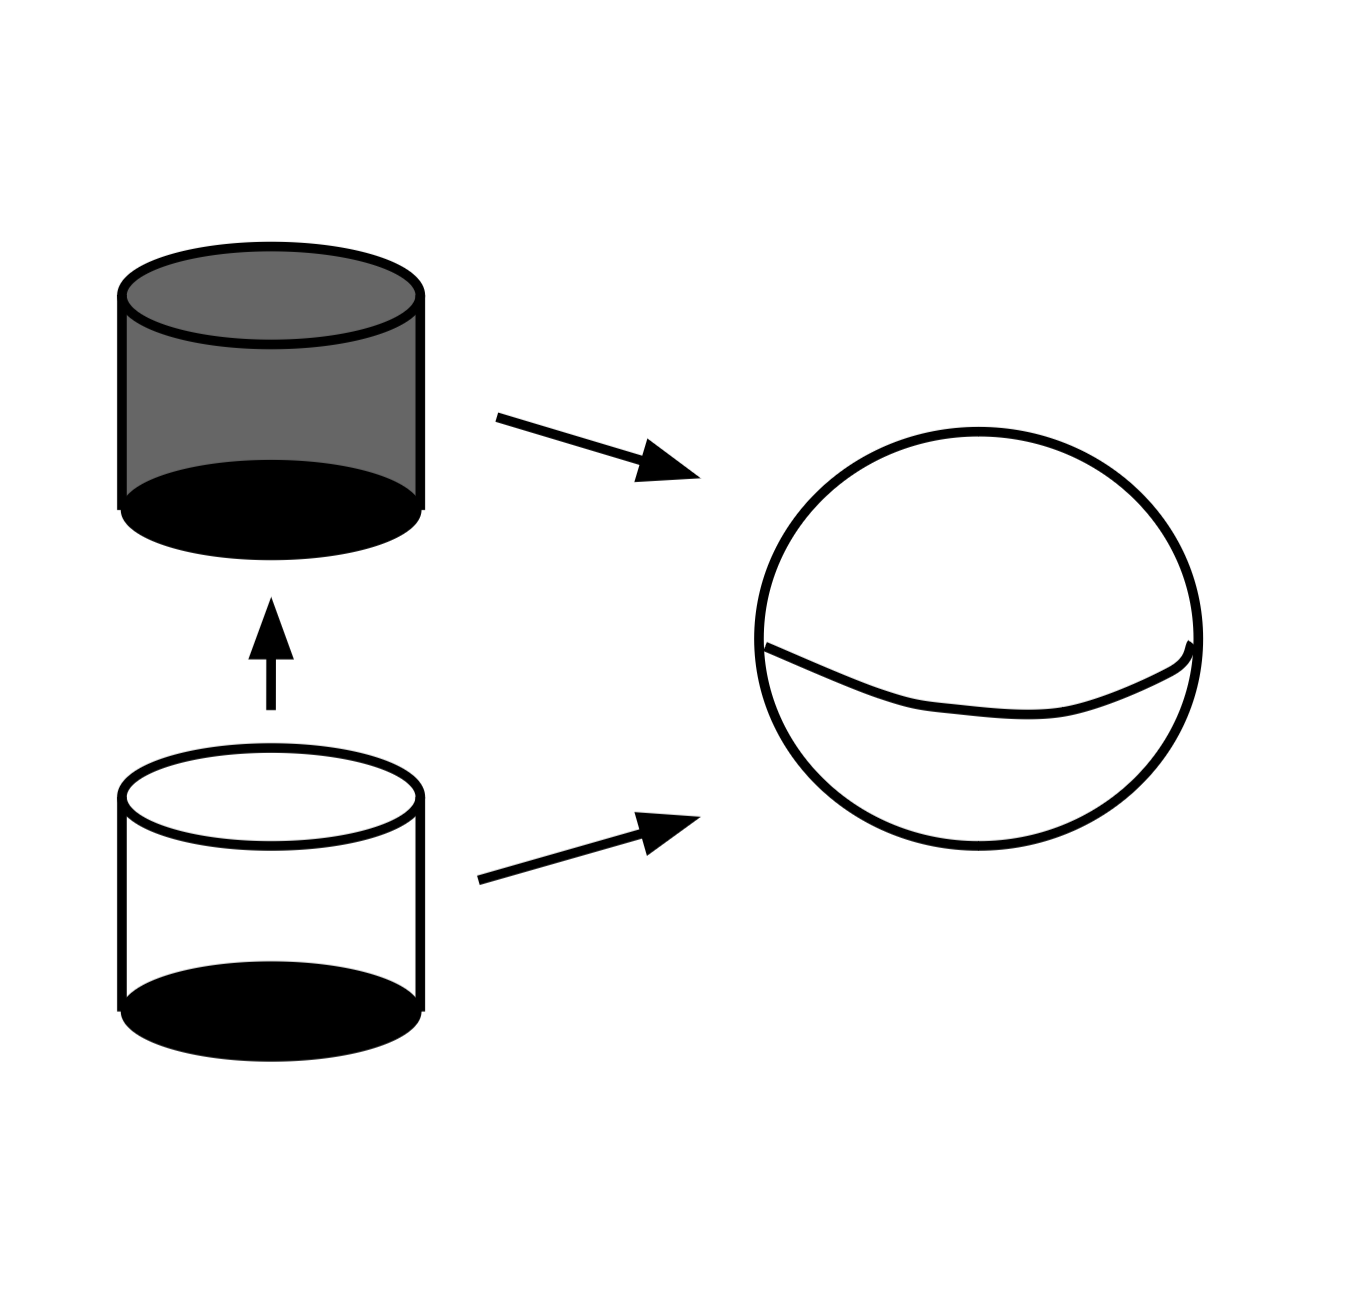
\includegraphics[width=0.5\textwidth]{HEP.png}
\end{center}

{\bf Prism Filling (PF)} Let Y be a quasicategory, and let f, g : ∂Δⁿ ⭢ Y. A homotopy h : ∂Δⁿ × Δ¹ ⭢ Y between f, g : ∂Δⁿ ⭢ Y extends to a map H : Δⁿ × Δ¹ ⭢ Y; this follows from the condition that Y be a quasicategory. H(-,1) and g match on ∂Δⁿ, producing a map f : X ⭢ Y, where X consists of two copies of Δⁿ glued together at the boundary. Consider a space X' formed as a quotient of Δⁿ × Δ¹ by ∂Δⁿ × Δ¹. There is a map φ : X ⭢ X'. An induction hypothesis on f and g involving πₙ ensures that the aparent map X ⭢ Y lifts along φ, producing a map from Δⁿ × Δ¹ which is constant on ∂Δⁿ × Δ¹. Stacking this on top of H can be done using an isomorphism between Δ¹ and Δ¹ glued with itself along different endpoints. Altogether this produces a homotopy between f and g.\\

Directed prism filling may combine fruitfully with the yoneda lemma and/or the fact that simplicial sets are determined by the sets [Δⁿ,X] along with combinatorial information (face and degeneracy maps).

{\bf Decomposing Δⁿ × Δ¹ into a colimit involving n+1 Δ${}^{n+1}$'s} ...

\begin{center}
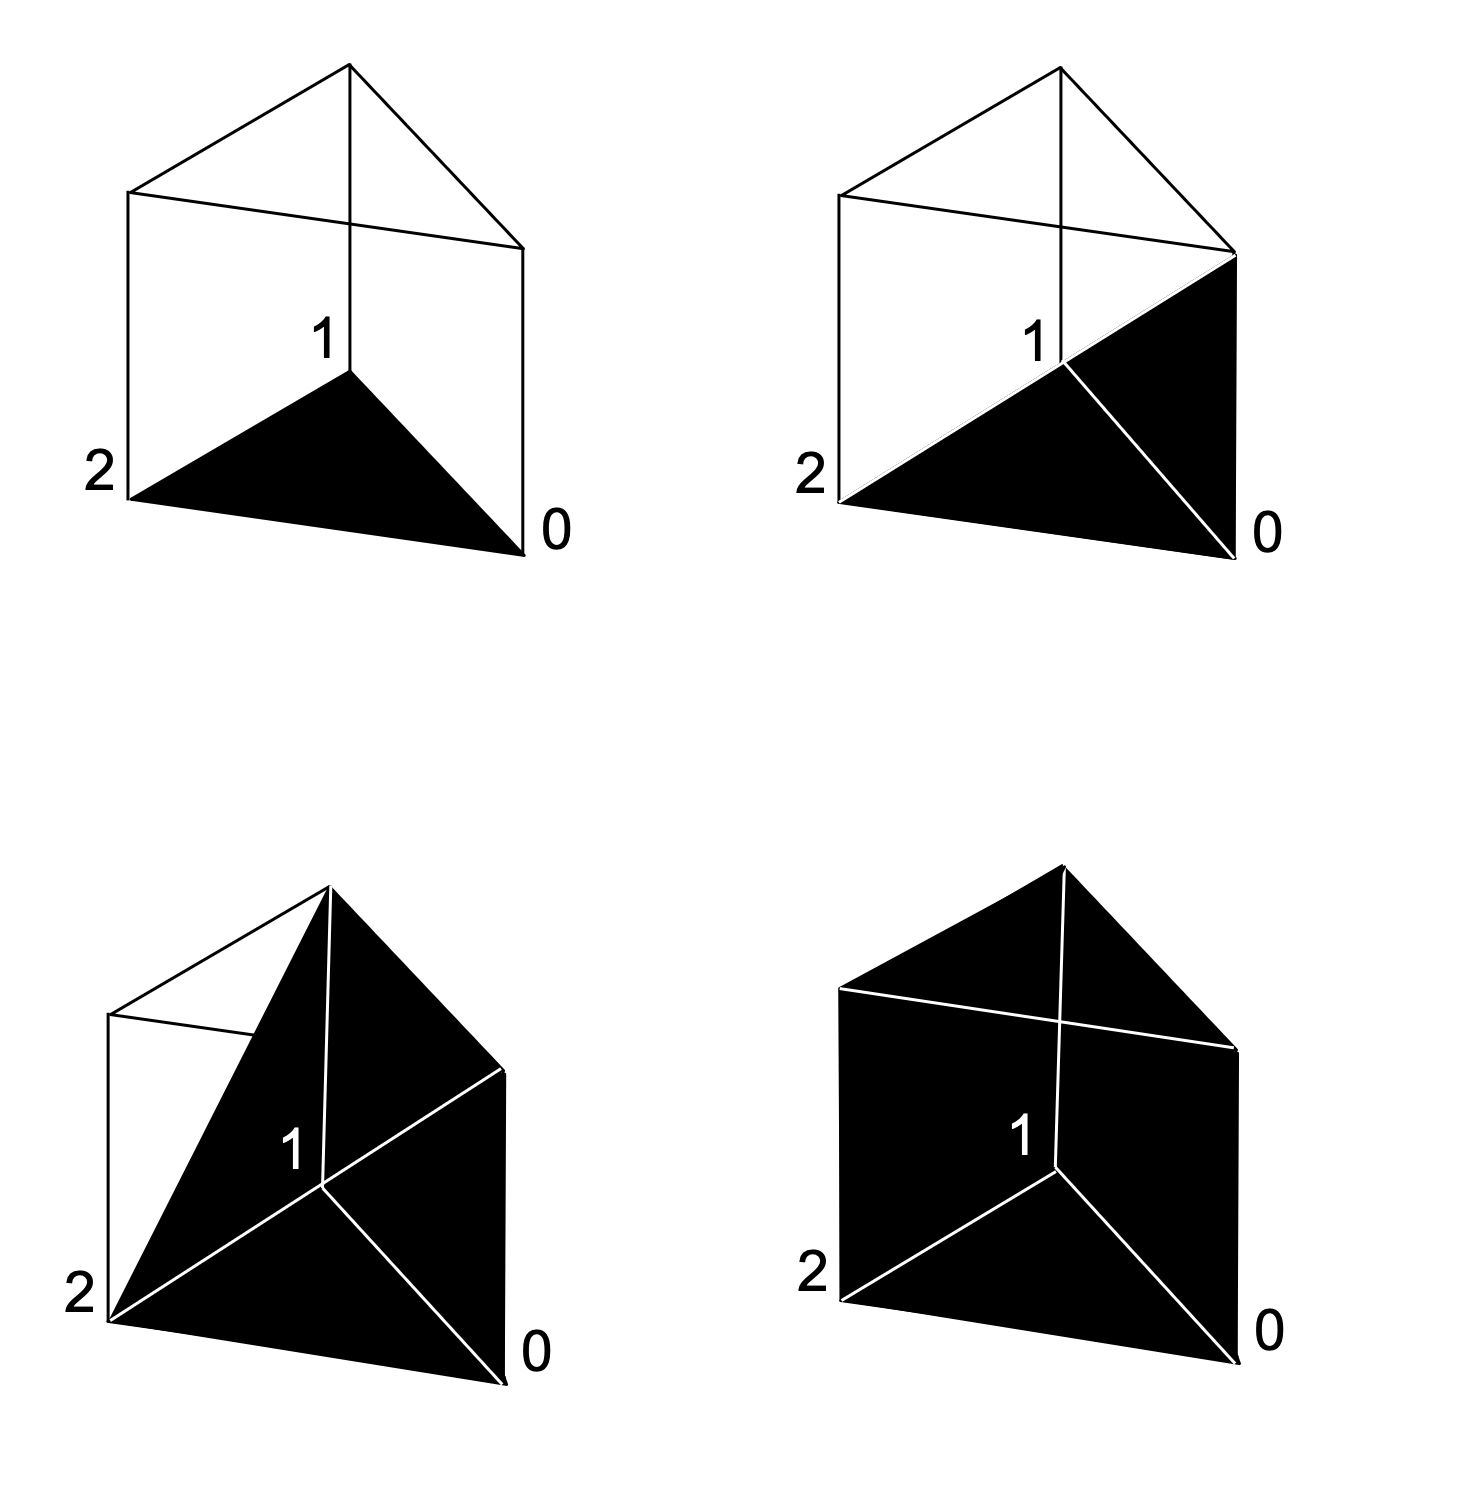
\includegraphics[width=300pt]{prismfilling.png}
\end{center}

In the above, it may be easier if we make use of sub-simplicial sets and prove the theorem using that colimit applied to a natural isomorphism of diagrams products an isomorphism.\\

The decomposition 

A definition of π⃗ₙ which is consistent with our goals of Wa and Pa is one as a certain pushout involving (Ω⃗ⁿ X)-- one which amounts to taking an equivalence relation by paths in Ω⃗ⁿ X which restrict to constant paths along the face maps fᵢ : Ω⃗${}^{n-1}$ X ⭢ Ω⃗ⁿ X. Here, Ω⃗ is easy to define in the model of quasi-categories, and it amounts . Besides fullfilling our goal of the first Whitehead theorem and puppe sequence, this definition of π⃗ₙ strikes me as elegant because it uses all of the ways for Ω⃗ⁿ X to map into Ω⃗${}^{n+1}$ X.\\

The next symbols in the project's ``periodic table" that we construct, after Ω⃗ and π⃗ₙ, will be B⃗ and E⃗, which we feature in the chapter on Puppe sequence (a).\\

A useful thing for us to construct first is the boundary of a product of Δ¹'s and the boundary of a directed simplex. We might even like to expand on this later, but for now just consider for a moment how each might be made out of a glueing construction involving face maps.\\

Even though the π⃗ₙ's can be defined using Ω⃗ⁿ X and various face maps f$\_(n,b)$ : Ω⃗${}^{n-1}$ X ⭢ Ω⃗${}^{n}$ X for $b : \{ 0, 1 \}$, it may be nice to have this as a result, with the definition one featuring two cubes glued together along their boundary.\\

This means that we want directed box filling in addition to directed prism filling (but which also uses directed prism filling in its proof).

{\bf Box Filling (BF)} Let Y be a quasicategory, and let f, g : ∂Δⁿ ⭢ Y. A homotopy h : ∂Δⁿ × Δ¹ ⭢ Y between f, g : ∂Δⁿ ⭢ Y extends to a map H : Δⁿ × Δ¹ ⭢ Y; this follows from the condition that Y be a quasicategory. H(-,1) and g match on ∂Δⁿ, producing a map f : X ⭢ Y, where X consists of two copies of Δⁿ glued together at the boundary. Consider a space X' formed as a quotient of Δⁿ × Δ¹ by ∂Δⁿ × Δ¹. There is a map φ : X ⭢ X'. An induction hypothesis on f and g involving πₙ ensures that the aparent map X ⭢ Y lifts along φ, producing a map from Δⁿ × Δ¹ which is constant on ∂Δⁿ × Δ¹. Stacking this on top of H can be done using an isomorphism between Δ¹ and Δ¹ glued with itself along different endpoints. Altogether this produces a homotopy between f and g.\\

This goes hand-in-hand with a definition of π⃗ₙ which suits (I) and (II) in the introduction to chapter (3). If we make sure to prove lemmas... 

The box filling and prism filling HEPs can be extended to the case of attaching all cells of a particular fixed dimension and as indexed by simplicial set arising from a set (or Lean 4 $\texttt{Type}$). That is, we might like to extend × $()$ (or possibly somehow a $\texttt{Set}$ as well), and that we may find an interest in the following two definitions of π⃗ₙ, which are designed to fullfill both (I) and (II) in the chapter's introduction.\\

Breaking down BF further can be done conveniently using sub-simplicial sets, just like we used in the proof of prism filling. 

\begin{center}
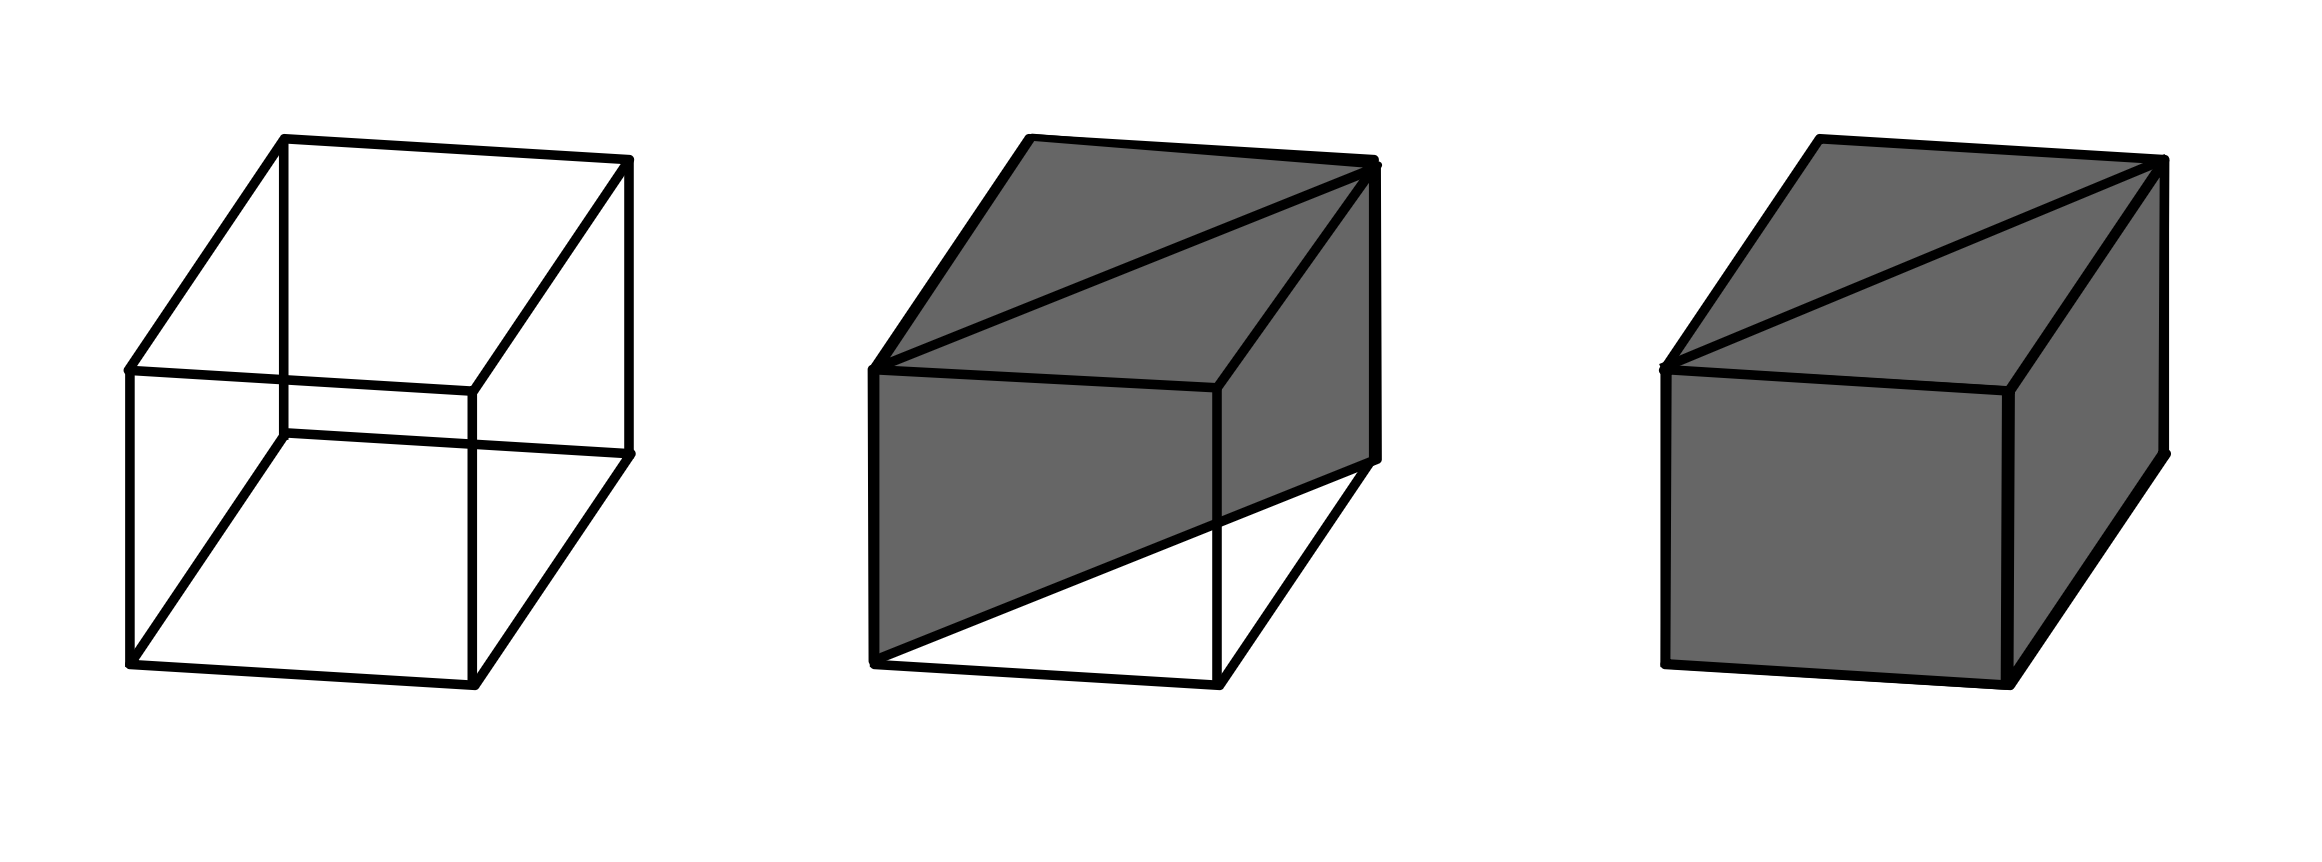
\includegraphics[width=300pt]{boxfilling.png}
\end{center}


{\bf Decomposing (Δ¹)ⁿ into a colimit involving n! Δⁿ's} Consider the face maps fᵢ : Δⁿ ⭢ Δ${}^{n+1}$


The decomposition 
The box filling lemma allows us to prove HEP:


\section{The Whitehead Theorem for ∞-Cat}

The HEP in the last 

..H(-,1) and g match on ∂Δⁿ, producing a map f : X ⭢ Y, where X consists of two copies of Δⁿ glued together at the boundary. Consider a space X' formed as a quotient of Δⁿ × Δ¹ by ∂Δⁿ × Δ¹. There is a map φ : X ⭢ X'. An induction hypothesis on f and g involving πₙ ensures that the aparent map X ⭢ Y lifts along φ, producing a map from Δⁿ × Δ¹ which is constant on ∂Δⁿ × Δ¹. Stacking this on top of H can be done using an isomorphism between Δ¹ and Δ¹ glued with itself along different endpoints. Altogether this produces a homotopy between f and g.\\

Imagine 


\chapter{Chapter 15: The Category of Pairs of ∞-Categories}

...\\


\chapter{Chapter 16: Internal and Operadic Categories and their Presheaves}

\iffalse
An operadic category is an algebra for the little rays operoid with 7 entries

An operadic internal category in C is an algebra in C for the little rays internal operoid with 13 entries

\fi

In this chapter, we discuss internal categories and internal presheaves in a pullback system. We may keep in mind that internal categories and internal presheaves can be formed in any category with pullbacks, even though we focus on the case of pullback systems because of our interest in Whitehead theorem (a).\\

After defining the category of internal categories D(Γ), we proceed to observe how, for C , D : D(Γ), F : C ⭢ D, (ω⃗ F).obj F forms an internal categry. Further, in considering internal (P⃗\_(Γ) F)-presheaves for  C , D : D(Γ), F : C ⭢ D, we proceed to make observations about (ω⃗ F).obj G.\\

{
\footnotesize
\begin{center}
\begin{tabular}{||l || l ||} 
 \hline
 $\texttt{Section}$  &\ $\texttt{Description}$ \\
 \hline \hline
 $\texttt{InternalCategory Γ : Cat}$   &\ Internal categories \\ 
 \hline
 $\texttt{InternalPresheaf Γ C : Cat}$ &\ Internal C-presheaves \\ 
 \hline
 The internal category principal &\ \texttt{f ×\_(B) f} forms an internal category\\
 \hline
 The internal presheaf principal &\ \texttt{f ×\_(B) g} forms an internal presheaf\\
 \hline
 P⃗ C : InternalCategory D(∞-Cat) &\ Ω⃗ C forms a component of an internal category \\
 \hline
 p⃗ (𝟙 C) D : InternalPresheaf D(∞-Cat⁄C) (P⃗ C) &\ ω⃗ (𝟙 C) D forms a component of an internal C-presheaf \\
 \hline
\end{tabular}
\end{center}
}



\iffalse

Definition of an operad ()
Definition of an 
Algebras for the little rays operoid
Algebras for the little lines operoid
Algebras for the little rays operad
Algebras for the little lines operad
\fi

\section{\texttt{Internal Categories}}

In this section I define an \href{https://ncatlab.org/nlab/show/internal+category}{internal category}, which structure plays a central role in \href{https://github.com/linlib/TheWhiteheadTheoremandTwoVariations/blob/main/Galois%20Theories%20Chapter%207%20(Janelidze%20and%20Borceux).pdf}{$\textit{Galois Theories}$} by Janelidze and Borceux.\\

Recall that, for a category C, with objects X${}_1$, X${}_2$, Y : C and morphisms $f_1$ : C.Hom X${}_1$ Y and $f_2$ : C.Hom X${}_2$ Y a pullback consists of:

\begin{definition}[Pullback] 
\begin{enumerate}
\item An object $\texttt{(pullback f_1 f_2).Obj : C}$
\item A morphism $\texttt{Pr}_1$ $\texttt{C.Hom (pullback f_1 f_2).Obj X}$${}_1$ 
\item A morphism $\texttt{Pr}_2$ $\texttt{C.Hom (pullback f_1 f_2).Obj X}$${}_2$ 
\item An equality $\texttt{Eqn :} \texttt{Pr}_1 \texttt{f}_1 = \texttt{Pr}_2 \texttt{f}_2$
\item A  of type 
\end{enumerate}
such that, for each object $\texttt{X : C}$ and each pair of morphisms $\texttt{g}_1 : C.Hom X X_1$, $\texttt{g}_1 : C.Hom X X_2$ such that $\texttt{f}_1 • \texttt{g}_1 = \texttt{f}_2 • \texttt{g}_2$, there is a unique $\texttt{h : C.Hom X (pullback f g).Obj}$ such that:
\begin{enumerate}
\item 
\item
\end{enumerate}
\end{enumerate}

In $\texttt{Categories and Hilbert Spaces}$, this was implemented as :



Let C be a category. An internal category ℂ consists of:

\begin{definition}[Internal Category] 
\begin{enumerate}
\item An object $\texttt{ℂ.Obj : ℂ}$
\item An object $\texttt{ℂ.Mor : ℂ}$ 
\item A morphism $\texttt{ℂ.Cod : C.Hom ℂ.Mor ℂ.Obj}$
\item A morphism $\texttt{ℂ.Dom : C.Hom ℂ.Mor ℂ.Obj}$
\item A morphism $\texttt{ℂ.Idn : C.Hom ℂ.Obj ℂ.Mor}$
\item A term $\texttt{X : (pullback ℂ.Dom ℂ.Cod)}$
\item A morphism $\texttt{ℂ.Mul : C.Hom X.Obj ℂ.Mul}$
\end{enumerate}
such that, writing $\texttt{g ∘\_(C) f}$ for $\texttt{C.Cmp X Y Z f g}$ and $\texttt{𝟙\_(X)}$ for $\texttt{C.Idn X}$,
\begin{enumerate}
\item $\texttt{∀(X:Obj),∀(Y:Obj),∀(f:Hom X Y),}$
\[\texttt{f ∘\_(C) (Idn X)\ =\ f}\]
\item $\texttt{∀(X:Obj),∀(Y:Obj),∀(f:Hom X Y),}$
\[\texttt{(Idn X) ∘\_(C) f\ =\ f}\]
\item $\texttt{∀(W:Obj),∀(X:Obj),∀(Y:Obj),∀(Z:Obj),}$ $\texttt{∀(f:Hom W X),}$ $\texttt{∀(g:Hom X Y),}$\\ $\texttt{∀(h:Hom Y Z),}$
\[\texttt{ f ∘\_(C) (g ∘\_(C) h) = (f ∘\_(C) g) ∘\_(C) h} \]
\end{enumerate}
\end{definition}

Discounting those entries of the internal category structure which assume the existence of pullbacks, an internal category has 13 entries. Internal categories are often defined on categories with $\textit{all pullbacks}$, but here we take an approach in which $\texttt{InternalCategory}$ has type $\texttt{Cat → Cat}$, so that it can be iterated. This entails separate entries assuming the existence of particular pullbacks.\\

%LEAN: definition of an internal category in a pullback system
\begin{center}
\begin{tcolorbox}[width=5in,colback={white},title={\begin{center}\texttt{Lean \thelcounter} \addtocounter{lcounter}{1}  \end{center}},colbacktitle=Blue,coltitle=black]
\begin{minted}[breaklines, escapeinside=||]{lean}

-- definition of an internal category in a pullback system
/-
structure internal_category (Γ : Cat) where
  Obj : .Obj
  Mor : .Obj
  Dom : .Hom Mor Obj
  Cod : .Hom Mor Obj
  Idn : .Hom Obj Mor
  Fst : .Cmp Obj Mor Obj Idn Dom  = 𝟙_(Γ.Obj) Obj
  Snd : .Cmp Obj Mor Obj Idn Cod = 𝟙_(Γ.Obj) Obj
--  Cmp : D(Γ).Γ.PulObj ...
-- Id₁ : D(Γ).
-- Id₂ : D(Γ).
-- Ass : D(Γ).
-/

\end{minted}
\end{tcolorbox}
\end{center}

The internal functor structure combines with the internal category structure to give a category of internal categories in a pullback system.\\

%LEAN: definition of an internal functor in a pullback system
\begin{center}
\begin{tcolorbox}[width=5in,colback={white},title={\begin{center}\texttt{Lean \thelcounter} \addtocounter{lcounter}{1}  \end{center}},colbacktitle=Blue,coltitle=black]
\begin{minted}[breaklines, escapeinside=||]{lean}

-- definition of an internal functor in a pullback system
structure internal_functor (Γ : pullback_system) (C : internal_category Γ) (D : internal_category Γ) where
  Obj : D(Γ).Hom C.Obj D.Obj
-- Mor : D(Γ).
-- Fst : D(Γ).
-- Snd : D(Γ).
-- Idn : D(Γ).
-- Cmp : D(Γ).

\end{minted}
\end{tcolorbox}
\end{center}


%LEAN: definition of the identity internal functor in a pullback system
\begin{center}
\begin{tcolorbox}[width=5in,colback={white},title={\begin{center}\texttt{Lean \thelcounter} \addtocounter{lcounter}{1}  \end{center}},colbacktitle=Blue,coltitle=black]
\begin{minted}[breaklines, escapeinside=||]{lean}

-- definition of the identity internal functor in a pullback system
def InternalCategoryIdn (Γ : pullback_system) (C : internal_category Γ) : (internal_functor Γ C C) := sorry

\end{minted}
\end{tcolorbox}
\end{center}

%LEAN: definition of the composition of internal functors in a pullback system
\begin{center}
\begin{tcolorbox}[width=5in,colback={white},title={\begin{center}\texttt{Lean \thelcounter} \addtocounter{lcounter}{1}  \end{center}},colbacktitle=Blue,coltitle=black]
\begin{minted}[breaklines, escapeinside=||]{lean}

-- definition of the composition of internal functors in a pullback system
def InternalCategoryCmp (Γ : pullback_system) (C : internal_category Γ) (D : internal_category Γ) (E : internal_category Γ) (F : internal_functor Γ C D) (G : internal_functor Γ D E) : (internal_functor Γ C E) := sorry

\end{minted}
\end{tcolorbox}
\end{center}

%LEAN: proving the first identity law for internal categories in a pullback system
\begin{center}
\begin{tcolorbox}[width=5in,colback={white},title={\begin{center}\texttt{Lean \thelcounter} \addtocounter{lcounter}{1}  \end{center}},colbacktitle=Blue,coltitle=black]
\begin{minted}[breaklines, escapeinside=||]{lean}

-- proving the the first identity law for internal categories in a pullback system
def InternalCategoryId₁ (Γ : pullback_system) (X : internal_category Γ) (Y : internal_category Γ) (f : internal_functor Γ X Y) : InternalCategoryCmp Γ X Y Y f (InternalCategoryIdn Γ Y) = f := sorry

\end{minted}
\end{tcolorbox}
\end{center}

%LEAN: proving the second identity law for internal categories  in a pullback system
\begin{center}
\begin{tcolorbox}[width=5in,colback={white},title={\begin{center}\texttt{Lean \thelcounter} \addtocounter{lcounter}{1}  \end{center}},colbacktitle=Blue,coltitle=black]
\begin{minted}[breaklines, escapeinside=||]{lean}

-- proving the second identity law for internal categories in a pullback system
def InternalCategoryId₂ (Γ : pullback_system) (X : internal_category Γ) (Y : internal_category Γ) (f : internal_functor Γ X Y) : (InternalCategoryCmp Γ X X Y (InternalCategoryIdn Γ X) f = f) := sorry

\end{minted}
\end{tcolorbox}
\end{center}

%LEAN: proving the associativity law for internal categories in a pullback system
\begin{center}
\begin{tcolorbox}[width=5in,colback={white},title={\begin{center}\texttt{Lean \thelcounter} \addtocounter{lcounter}{1}  \end{center}},colbacktitle=Blue,coltitle=black]
\begin{minted}[breaklines, escapeinside=||]{lean}

-- proving the associativity law for internal categories in a pullback system
def InternalCategoryAss (Γ : pullback_system) (W : internal_category Γ) (X : internal_category Γ) (Y : internal_category Γ) (Z  : internal_category Γ) (f : internal_functor Γ W X) (g : internal_functor Γ X Y) (h : internal_functor Γ Y Z) : InternalCategoryCmp Γ W X Z f (InternalCategoryCmp Γ X Y Z g h) = InternalCategoryCmp Γ W Y Z (InternalCategoryCmp Γ W X Y f g) h := sorry

\end{minted}
\end{tcolorbox}
\end{center}

%LEAN: defining the category of internal categories in a pullback system
\begin{center}
\begin{tcolorbox}[width=5in,colback={white},title={\begin{center}\texttt{Lean \thelcounter} \addtocounter{lcounter}{1}  \end{center}},colbacktitle=Blue,coltitle=black]
\begin{minted}[breaklines, escapeinside=||]{lean}

/-
def InternalCategory (Γ : pulback_system) : 𝐂𝐚𝐭.Obj := {Obj := internal_category Γ, Hom := internal_functor Γ, Idn := InternalCategoryIdn Γ, Cmp := InternalCategoryCmp Γ, Id₁ := InternalCategoryId₁ Γ, Id₂ := InternalCategoryId₂ Γ, Ass := InternalCategoryAss Γ}
-/

\end{minted}
\end{tcolorbox}
\end{center}

%LEAN: 
\begin{center}
\begin{tcolorbox}[width=5in,colback={white},title={\begin{center}\texttt{Lean \thelcounter} \addtocounter{lcounter}{1}  \end{center}},colbacktitle=Blue,coltitle=black]
\begin{minted}[breaklines, escapeinside=||]{lean}

-- notation : 2000 "Cat_(" Γ ")" => InternalCategory Γ

\end{minted}
\end{tcolorbox}
\end{center}

\section{\texttt{Internal Presheaves}}

An internal presheaf consists of:

\iffalse
\begin{definition}[Internal Presheaf]
  \begin{enumerate}
  \item A class $\texttt{C.Obj}$ of objects
  \item For each pair of objects $\texttt{X,Y:Obj}$, a class 
  \[ \texttt{C.Hom X,Y} \] 
  whose elements are called maps or morphisms. 
  \item For each object $\texttt{X}$, a morphism 
  \[ \texttt{C.Idn X} \]
  \item For each triple of objects $\texttt{X, Y, Z : Obj}$, a function 
  \[ \texttt{C.Cmp X Y Z : (C.Hom X Y) → (C.Hom Y Z) → (C.Hom X Z)} \]
  \end{enumerate}
  such that, writing $\texttt{g ∘\_(C) f}$ for $\texttt{C.Cmp X Y Z f g}$ and $\texttt{𝟙\_(X)}$ for $\texttt{C.Idn X}$,
  \begin{enumerate}
  \item $\texttt{∀(X:Obj),∀(Y:Obj),∀(f:Hom X Y),}$
  \[\texttt{f ∘\_(C) (Idn X)\ =\ f}\]
  \item $\texttt{∀(X:Obj),∀(Y:Obj),∀(f:Hom X Y),}$
  \[\texttt{(Idn X) ∘\_(C) f\ =\ f}\]
  \item $\texttt{∀(W:Obj),∀(X:Obj),∀(Y:Obj),∀(Z:Obj),}$ $\texttt{∀(f:Hom W X),}$ $\texttt{∀(g:Hom X Y),}$\\ $\texttt{∀(h:Hom Y Z),}$
  \[\texttt{ f ∘\_(C) (g ∘\_(C) h) = (f ∘\_(C) g) ∘\_(C) h} \]
  \end{enumerate}
  \end{definition}
\fi



\section{The P⃗ and O⃗ Functors}

In this section we mention the internal category principal, which says that the pullback of any morphism with itself forms a component of an internal category in any category in which this pullback exists. In fact, the most general form of the theorem works for a noncommutative analogue of pullback.\\ 


\section{The p⃗ and o⃗ Functors}

Next we mention the internal presheaf principal, which says that the pullback of any morphism with another forms a component of an internal presheaf in any category with pullbacks. Just as is the case for the last theorem, the most general form of this idea works for non-commutative analogues of pullback, wheras the case of pullback gives an internal groupoid action.\\





\newpage
{
\Huge 
\begin{center}
\ \\
\ \\
\texttt{Bibliography}
\ \\
\ \\
\end{center}
\thispagestyle{empty}
}

\iffalse
Needs citation:

Pure Galois theory in categories (Janelidze) https://scholar.google.com/citations?view_op=view_citation&hl=en&user=fOYPVWwAAAAJ&citation_for_view=fOYPVWwAAAAJ:9yKSN-GCB0IC
\item Facets of descent I (Janelidze) https://scholar.google.com/citations?view_op=view_citation&hl=en&user=fOYPVWwAAAAJ&citation_for_view=fOYPVWwAAAAJ:2osOgNQ5qMEC
\item Internal object actions (Janelidze) https://scholar.google.com/citations?view_op=view_citation&hl=en&user=fOYPVWwAAAAJ&citation_for_view=fOYPVWwAAAAJ:zYLM7Y9cAGgC

\fi




\begin{enumerate}
\item Davis, James F., and Paul Kirk. Lecture notes in algebraic topology. Vol. 35. Providence: American Mathematical Society, 2001.
\item \iffalse \url{https://florisvandoorn.com/papers/dissertation.pdf} \fi
\item Galois theory and a general notion of central simple extension (Janelidze) \iffalse https://scholar.google.com/citations?view_op=view_citation&hl=en&user=fOYPVWwAAAAJ&citation_for_view=fOYPVWwAAAAJ:d1gkVwhDpl0C \fi
\item Borceux, F., and Janelidze, G. Galois Theories. Cambridge Studies in Advanced Mathematics, vol. 72. Cambridge University Press, Cambridge, 2001. ISBN 0-521-80309-8.
\item Tom Leinster, Higher Operads, Higher Categories, London Mathematical Society Lecture Note Series, vol. 298, Cambridge University Press, 2004.
\item Lurie, Jacob. Higher Topos Theory. Annals of Mathematics Studies, vol. 170. Princeton University Press, Princeton, NJ, 2009.
\item Leonardo de Moura and Jeremy Avigad, ``The Lean Theorem Prover," Journal of Formalized Reasoning, vol. 8, no. 1, pp. 1-37, 2015.
\item Leonardo de Moura and Soonho Kong, ``Lean Theorem Proving Tutorial," Proceedings of the 6th International Conference on Interactive Theorem Proving (ITP), Lecture Notes in Computer Science, vol. 9236, pp. 378-395, Springer, Berlin, 2015.
\item Jeremy Avigad, Leonardo de Moura, and Soonho Kong, ``Theorem Proving in Lean," Logical Methods in Computer Science, vol. 12, no. 4, pp. 1-43, 2016.
\item Daniel Selsam, Leonardo de Moura, David L. Dill, and David L. Vlah, ``Leonardo: A Solver for MIP and Mixed Integer Nonlinear Programming," Proceedings of the 33rd Conference on Neural Information Processing Systems (NeurIPS), pp. 493-504, 2019.
\item \url{https://www.uni-muenster.de/IVV5WS/WebHop/user/nikolaus/Papers/oo-bundles_general_theory.pdf}
\item \url{https://www.cse.chalmers.se/~coquand/cubicaltt.pdf}
\item \url{https://arxiv.org/pdf/1607.04156.pdf}
\item \url{https://carloangiuli.com}
\end{enumerate}

Further reading:

\begin{enumerate}
\item J. Beck, ``Distributive laws," in Seminar on Triples and Categorical Homology Theory, Springer-Verlag, 1969, pp. 119-140.
\item Saunders Mac Lane, "Categories for the Working Mathematician," Graduate Texts in Mathematics, vol. 5, Springer-Verlag, New York, 1971.
\item Samuel Eilenberg and Saunders Mac Lane, ``General Theory of Natural Equivalences," Transactions of the American Mathematical Society, vol. 58, no. 2, pp. 231-294, 1945.
\item Daniel M. Kan, ``Adjoint Functors," Transactions of the American Mathematical Society, vol. 87, no. 2, pp. 294-329, 1958.
\item Chris Heunen, Jamie Vicary, and Stefan Wolf, ``Categories for Quantum Theory: An Introduction," Oxford Graduate Texts, Oxford University Press, Oxford, 2018.
\item S. Eilenberg and J. C. Moore, ``Adjoint Functors and Triples," Proceedings of the Conference on Categorical Algebra, La Jolla, California, 1965, pp. 89-106.
\item Daniel M. Kan, ``On Adjoints to Functors" (1958): In this paper, Kan further explored the theory of adjoint functors, focusing on the existence and uniqueness of adjoints. His work provided important insights into the fundamental aspects of adjoint functors and their role in category theory.
\item \href{https://mathematicswithoutapologies.wordpress.com/2015/05/13/univalent-foundations-no-comment/}{A comment thread concerning Jacob Lurie's breakthrough prize and different approaches to homotopy on the computer}
\item Arlin, Kevin David. "2-categorical Brown representability and the relation between derivators and infinity-categories." Doctoral dissertation, University of California, Los Angeles, 2020.
\item 
\end{enumerate}

Some lectures, videos, and Stackexchange questions:

\begin{enumerate}
\item \url{https://www.youtube.com/watch?v=Ob9tOgWumPI}
\item \url{https://www.youtube.com/watch?v=xYenPIeX6MY}
\item \url{https://mathoverflow.net/questions/5901/do-the-signs-in-puppe-sequences-matter}
\end{enumerate}

\iffalse
Maintainers:

For a list containing more detailed information, see https://leanprover-community.github.io/teams/maintainers.html

https://www.youtube.com/watch?v=6FLmQwhQlwA
https://www.youtube.com/watch?v=kjBDkH10OnQ
https://www.birs.ca/events/2023/5-day-workshops/23w5124/videos/watch/202305241110-Riou.html
https://github.com/ADedecker/gauss
https://github.com/ADedecker/amenable

\fi


Ideas for future applications:

\begin{enumerate}
\item \url{https://arxiv.org/pdf/2206.13563.pdf}
\end{enumerate}

\newpage 
\ \\
\ \\
\ \\
\ \\
\ \\
\ \\
%LEAN: 
\begin{center}
\begin{tcolorbox}[width=5in,colback={white},title={\begin{center}\texttt{About the Author} \addtocounter{lcounter}{1}  \end{center}},colbacktitle=Yellow,coltitle=black]
Dean Young is a master's student at New York University, where he studies mathematics. \\
\begin{center}

\includegraphics[width=7.5cm,height=5cm]{about.jpg}
\end{center}
\end{tcolorbox}
\end{center}

\begin{center}
\begin{tcolorbox}[width=5in,colback={white},title={\begin{center}\texttt{About the Author} \addtocounter{lcounter}{1}  \end{center}},colbacktitle=Yellow,coltitle=black]
Jiazhen Xia is a graduate student at Zhejiang University, where he studies computer science. \\
\begin{center}

\includegraphics[width=7.5cm]{about2.jpg}
\end{center}
\end{tcolorbox}
\end{center}
\newpage
\ \\
\thispagestyle{empty}






\end{document}







































